\documentclass[twoside]{book}

% Packages required by doxygen
\usepackage{calc}
\usepackage{doxygen}
\usepackage{graphicx}
\usepackage[utf8]{inputenc}
\usepackage{makeidx}
\usepackage{multicol}
\usepackage{multirow}
\usepackage{textcomp}
\usepackage[table]{xcolor}

% Font selection
\usepackage[T1]{fontenc}
\usepackage{mathptmx}
\usepackage[scaled=.90]{helvet}
\usepackage{courier}
\usepackage{amssymb}
\usepackage{sectsty}
\renewcommand{\familydefault}{\sfdefault}
\allsectionsfont{%
  \fontseries{bc}\selectfont%
  \color{darkgray}%
}
\renewcommand{\DoxyLabelFont}{%
  \fontseries{bc}\selectfont%
  \color{darkgray}%
}

% Page & text layout
\usepackage{geometry}
\geometry{%
  a4paper,%
  top=2.5cm,%
  bottom=2.5cm,%
  left=2.5cm,%
  right=2.5cm%
}
\tolerance=750
\hfuzz=15pt
\hbadness=750
\setlength{\emergencystretch}{15pt}
\setlength{\parindent}{0cm}
\setlength{\parskip}{0.2cm}
\makeatletter
\renewcommand{\paragraph}{%
  \@startsection{paragraph}{4}{0ex}{-1.0ex}{1.0ex}{%
    \normalfont\normalsize\bfseries\SS@parafont%
  }%
}
\renewcommand{\subparagraph}{%
  \@startsection{subparagraph}{5}{0ex}{-1.0ex}{1.0ex}{%
    \normalfont\normalsize\bfseries\SS@subparafont%
  }%
}
\makeatother

% Headers & footers
\usepackage{fancyhdr}
\pagestyle{fancyplain}
\fancyhead[LE]{\fancyplain{}{\bfseries\thepage}}
\fancyhead[CE]{\fancyplain{}{}}
\fancyhead[RE]{\fancyplain{}{\bfseries\leftmark}}
\fancyhead[LO]{\fancyplain{}{\bfseries\rightmark}}
\fancyhead[CO]{\fancyplain{}{}}
\fancyhead[RO]{\fancyplain{}{\bfseries\thepage}}
\fancyfoot[LE]{\fancyplain{}{}}
\fancyfoot[CE]{\fancyplain{}{}}
\fancyfoot[RE]{\fancyplain{}{\bfseries\scriptsize Generated on Tue Jul 12 2016 14\-:15\-:10 for ec by Doxygen }}
\fancyfoot[LO]{\fancyplain{}{\bfseries\scriptsize Generated on Tue Jul 12 2016 14\-:15\-:10 for ec by Doxygen }}
\fancyfoot[CO]{\fancyplain{}{}}
\fancyfoot[RO]{\fancyplain{}{}}
\renewcommand{\footrulewidth}{0.4pt}
\renewcommand{\chaptermark}[1]{%
  \markboth{#1}{}%
}
\renewcommand{\sectionmark}[1]{%
  \markright{\thesection\ #1}%
}

% Indices & bibliography
\usepackage{natbib}
\usepackage[titles]{tocloft}
\setcounter{tocdepth}{3}
\setcounter{secnumdepth}{5}
\makeindex

% Hyperlinks (required, but should be loaded last)
\usepackage{ifpdf}
\ifpdf
  \usepackage[pdftex,pagebackref=true]{hyperref}
\else
  \usepackage[ps2pdf,pagebackref=true]{hyperref}
\fi
\hypersetup{%
  colorlinks=true,%
  linkcolor=blue,%
  citecolor=blue,%
  unicode%
}

% Custom commands
\newcommand{\clearemptydoublepage}{%
  \newpage{\pagestyle{empty}\cleardoublepage}%
}


%===== C O N T E N T S =====

\begin{document}

% Titlepage & ToC
\hypersetup{pageanchor=false}
\pagenumbering{roman}
\begin{titlepage}
\vspace*{7cm}
\begin{center}%
{\Large ec }\\
\vspace*{1cm}
{\large Generated by Doxygen 1.8.6}\\
\vspace*{0.5cm}
{\small Tue Jul 12 2016 14:15:10}\\
\end{center}
\end{titlepage}
\clearemptydoublepage
\tableofcontents
\clearemptydoublepage
\pagenumbering{arabic}
\hypersetup{pageanchor=true}

%--- Begin generated contents ---
\chapter{R\-E\-A\-D\-M\-E}
\label{md_README}
\hypertarget{md_README}{}
\#ec 
\chapter{Hierarchical Index}
\section{Class Hierarchy}
This inheritance list is sorted roughly, but not completely, alphabetically\-:\begin{DoxyCompactList}
\item \contentsline{section}{ec\-:\-:Async\-Context}{\pageref{structec_1_1AsyncContext}}{}
\item \contentsline{section}{ec\-:\-:Data}{\pageref{classec_1_1Data}}{}
\item \contentsline{section}{ec\-:\-:Date}{\pageref{classec_1_1Date}}{}
\item enable\-\_\-shared\-\_\-from\-\_\-this\begin{DoxyCompactList}
\item \contentsline{section}{ec\-:\-:Tcp\-Session}{\pageref{classec_1_1TcpSession}}{}
\end{DoxyCompactList}
\item \contentsline{section}{ec\-:\-:Extendable\-Single\-Queue$<$ T $>$}{\pageref{classec_1_1ExtendableSingleQueue}}{}
\item \contentsline{section}{ec\-:\-:Loop}{\pageref{classec_1_1Loop}}{}
\begin{DoxyCompactList}
\item \contentsline{section}{ec\-:\-:Tcp\-Server\-Dispatcher}{\pageref{classec_1_1TcpServerDispatcher}}{}
\end{DoxyCompactList}
\item \contentsline{section}{ec\-:\-:Tcp\-Server\-Dispatcher\-:\-:New\-Session\-Data}{\pageref{structec_1_1TcpServerDispatcher_1_1NewSessionData}}{}
\item \contentsline{section}{ec\-:\-:Safe\-Queue$<$ T $>$}{\pageref{classec_1_1SafeQueue}}{}
\item \contentsline{section}{ec\-:\-:Safe\-Queue$<$ ec\-:\-:ec\-:\-:Async\-Context $\ast$ $>$}{\pageref{classec_1_1SafeQueue}}{}
\item \contentsline{section}{ec\-:\-:Safe\-Queue$<$ ec\-:\-:ec\-:\-:Data $\ast$ $>$}{\pageref{classec_1_1SafeQueue}}{}
\item \contentsline{section}{ec\-:\-:Single\-Queue$<$ T $>$}{\pageref{classec_1_1SingleQueue}}{}
\item \contentsline{section}{Stream\-Reader}{\pageref{classStreamReader}}{}
\item \contentsline{section}{Stream\-Writer}{\pageref{classStreamWriter}}{}
\item T\begin{DoxyCompactList}
\item \contentsline{section}{ec\-:\-:Singleton$<$ T $>$}{\pageref{classec_1_1Singleton}}{}
\end{DoxyCompactList}
\item \contentsline{section}{ec\-:\-:Tcp\-Server}{\pageref{classec_1_1TcpServer}}{}
\item \contentsline{section}{ec\-:\-:Tcp\-Socket}{\pageref{classec_1_1TcpSocket}}{}
\begin{DoxyCompactList}
\item \contentsline{section}{ec\-:\-:Tcp\-Client}{\pageref{classec_1_1TcpClient}}{}
\item \contentsline{section}{ec\-:\-:Tcp\-Session}{\pageref{classec_1_1TcpSession}}{}
\end{DoxyCompactList}
\item \contentsline{section}{ec\-:\-:Time}{\pageref{classec_1_1Time}}{}
\item \contentsline{section}{ec\-:\-:Timer}{\pageref{classec_1_1Timer}}{}
\end{DoxyCompactList}

\chapter{Class Index}
\section{Class List}
Here are the classes, structs, unions and interfaces with brief descriptions\-:\begin{DoxyCompactList}
\item\contentsline{section}{\hyperlink{classec_1_1Date}{ec\-::\-Date} \\*日期类 }{\pageref{classec_1_1Date}}{}
\item\contentsline{section}{\hyperlink{classec_1_1FrameLoop}{ec\-::\-Frame\-Loop} \\*拥有幀定时器的事件循环 }{\pageref{classec_1_1FrameLoop}}{}
\item\contentsline{section}{\hyperlink{classec_1_1HttpRequest}{ec\-::\-Http\-Request} }{\pageref{classec_1_1HttpRequest}}{}
\item\contentsline{section}{\hyperlink{classec_1_1HttpServer}{ec\-::\-Http\-Server} }{\pageref{classec_1_1HttpServer}}{}
\item\contentsline{section}{\hyperlink{classec_1_1Loop}{ec\-::\-Loop} \\*事件循环,对event\-\_\-base的封装。 }{\pageref{classec_1_1Loop}}{}
\item\contentsline{section}{\hyperlink{classec_1_1TcpClient}{ec\-::\-Tcp\-Client} \\*客户端\-T\-C\-P连接 }{\pageref{classec_1_1TcpClient}}{}
\item\contentsline{section}{\hyperlink{classec_1_1TcpServer}{ec\-::\-Tcp\-Server} \\*T\-C\-P服务器 }{\pageref{classec_1_1TcpServer}}{}
\item\contentsline{section}{\hyperlink{classec_1_1TcpServerDispatcher}{ec\-::\-Tcp\-Server\-Dispatcher} \\*T\-C\-P服务器会话调度管理器 }{\pageref{classec_1_1TcpServerDispatcher}}{}
\item\contentsline{section}{\hyperlink{classec_1_1TcpSession}{ec\-::\-Tcp\-Session} \\*服务端\-T\-C\-P连接 }{\pageref{classec_1_1TcpSession}}{}
\item\contentsline{section}{\hyperlink{classec_1_1TcpSocket}{ec\-::\-Tcp\-Socket} \\*T\-C\-P连接基类 }{\pageref{classec_1_1TcpSocket}}{}
\item\contentsline{section}{\hyperlink{classec_1_1Time}{ec\-::\-Time} \\*时间类 }{\pageref{classec_1_1Time}}{}
\item\contentsline{section}{\hyperlink{classec_1_1Timer}{ec\-::\-Timer} \\*定时器类。 }{\pageref{classec_1_1Timer}}{}
\end{DoxyCompactList}

\chapter{Class Documentation}
\hypertarget{classec_1_1Date}{\section{ec\-:\-:Date Class Reference}
\label{classec_1_1Date}\index{ec\-::\-Date@{ec\-::\-Date}}
}


日期类  




{\ttfamily \#include $<$date.\-h$>$}

\subsection*{Public Member Functions}
\begin{DoxyCompactItemize}
\item 
\hyperlink{classec_1_1Date_a87b10f3e182109a78d3b68e9b1ed20e2}{Date} ()
\item 
\hyperlink{classec_1_1Date_a8862acf628e847927edaea397113036b}{Date} (time\-\_\-t \hyperlink{classec_1_1Date_ae376652bff3f8476f948c14cb00601c5}{stamp})
\item 
\hyperlink{classec_1_1Date_aa73c77460f766467202a9695b7b7649c}{Date} (const \hyperlink{classec_1_1Time}{Time} \&time)
\item 
\hypertarget{classec_1_1Date_ae3e63bec9accf142fe9a238a43e93626}{{\bfseries Date} (const \hyperlink{classec_1_1Date}{Date} \&date)}\label{classec_1_1Date_ae3e63bec9accf142fe9a238a43e93626}

\item 
\hyperlink{classec_1_1Date_a1dae4bdb08788d69fcbbb0a0233e27a1}{Date} (int \hyperlink{classec_1_1Date_ad8ff77d7111044313c6d07c1096c7330}{year}, int \hyperlink{classec_1_1Date_a8f1a6ea36ce7a64d2aa43c93a992bcd5}{month}, int \hyperlink{classec_1_1Date_a0544c98d04060feb7345092fb60b8065}{day}, int \hyperlink{classec_1_1Date_a5c5252eb904dba193e2347f955d986f6}{hour}=0, int \hyperlink{classec_1_1Date_a572776fe397fd2e25455f23a9de91d2d}{minute}=0, int \hyperlink{classec_1_1Date_a62f978e3fff3e38682bd9c4876beea5d}{second}=0)
\begin{DoxyCompactList}\small\item\em 以指定时间构造 \end{DoxyCompactList}\item 
void \hyperlink{classec_1_1Date_a991e12c24956f398a2d86ddaf8e99e2f}{set} (time\-\_\-t \hyperlink{classec_1_1Date_ae376652bff3f8476f948c14cb00601c5}{stamp})
\item 
\hyperlink{classec_1_1Date}{Date} \hyperlink{classec_1_1Date_ae94b1e3c919d58e5539088e863d1ba0d}{clone} () const 
\item 
time\-\_\-t \hyperlink{classec_1_1Date_ae376652bff3f8476f948c14cb00601c5}{stamp} () const 
\item 
time\-\_\-t \hyperlink{classec_1_1Date_ad9ef9967be21c60db8a78dc5d0e46ab4}{utc\-Stamp} () const 
\item 
\hyperlink{classec_1_1Time}{Time} \hyperlink{classec_1_1Date_a37f8cee14d869d9b132700f8568270de}{to\-Time} () const 
\item 
std\-::string \hyperlink{classec_1_1Date_a0566e90d744f4d1d8d5490a9be7a5bbc}{to\-String} () const 
\item 
int \hyperlink{classec_1_1Date_ad8ff77d7111044313c6d07c1096c7330}{year} () const 
\item 
int \hyperlink{classec_1_1Date_a8f1a6ea36ce7a64d2aa43c93a992bcd5}{month} () const 
\item 
int \hyperlink{classec_1_1Date_a0544c98d04060feb7345092fb60b8065}{day} () const 
\item 
int \hyperlink{classec_1_1Date_a5c5252eb904dba193e2347f955d986f6}{hour} () const 
\item 
int \hyperlink{classec_1_1Date_a572776fe397fd2e25455f23a9de91d2d}{minute} () const 
\item 
int \hyperlink{classec_1_1Date_a62f978e3fff3e38682bd9c4876beea5d}{second} () const 
\item 
int \hyperlink{classec_1_1Date_a9fd30981481e444ae07f908b447ce639}{week} () const 
\item 
int \hyperlink{classec_1_1Date_a02c5f9f15c4316e6a46d4ee113ab1b15}{year\-Day} () const 
\item 
\hyperlink{classec_1_1Date}{Date} \& \hyperlink{classec_1_1Date_a9a89c8fd2f2244a6524f0149c31f51f1}{set\-Year} (int \hyperlink{classec_1_1Date_ad8ff77d7111044313c6d07c1096c7330}{year})
\item 
\hyperlink{classec_1_1Date}{Date} \& \hyperlink{classec_1_1Date_a9de7e244d6d3c0b934c8226ec2a58eb4}{set\-Month} (int \hyperlink{classec_1_1Date_a8f1a6ea36ce7a64d2aa43c93a992bcd5}{month})
\item 
\hyperlink{classec_1_1Date}{Date} \& \hyperlink{classec_1_1Date_a6e0b3d8c7e82d8d5e0367e3aaf5753e6}{set\-Day} (int \hyperlink{classec_1_1Date_a0544c98d04060feb7345092fb60b8065}{day})
\item 
\hyperlink{classec_1_1Date}{Date} \& \hyperlink{classec_1_1Date_ace13c15d6883dfdddef61dfaca003a46}{set\-Hour} (int \hyperlink{classec_1_1Date_a5c5252eb904dba193e2347f955d986f6}{hour})
\item 
\hyperlink{classec_1_1Date}{Date} \& \hyperlink{classec_1_1Date_aca4de51e0906fa33907044f3ac4747b7}{set\-Minute} (int \hyperlink{classec_1_1Date_a572776fe397fd2e25455f23a9de91d2d}{minute})
\item 
\hyperlink{classec_1_1Date}{Date} \& \hyperlink{classec_1_1Date_a2dd73608deaa5f29c14a558190c9a232}{set\-Second} (int \hyperlink{classec_1_1Date_a62f978e3fff3e38682bd9c4876beea5d}{second})
\item 
\hyperlink{classec_1_1Date}{Date} \& \hyperlink{classec_1_1Date_a62f053cb6c9e23173b494fd420c58b7b}{add\-Year} (int \hyperlink{classec_1_1Date_ad8ff77d7111044313c6d07c1096c7330}{year})
\item 
\hyperlink{classec_1_1Date}{Date} \& \hyperlink{classec_1_1Date_a8611507e4a92fd7abd0b5ba9a3503c1c}{add\-Month} (int \hyperlink{classec_1_1Date_a8f1a6ea36ce7a64d2aa43c93a992bcd5}{month})
\item 
\hyperlink{classec_1_1Date}{Date} \& \hyperlink{classec_1_1Date_ae0903b4862d9ffdda4308a7b403235f3}{add\-Second} (int \hyperlink{classec_1_1Date_a62f978e3fff3e38682bd9c4876beea5d}{second})
\item 
\hyperlink{classec_1_1Date}{Date} \& \hyperlink{classec_1_1Date_a199dad3bfafc2cb4d16bff81683d6cca}{sharp\-Year} ()
\item 
\hyperlink{classec_1_1Date}{Date} \& \hyperlink{classec_1_1Date_a29f26d3467fcc160ec499da528ddac03}{sharp\-Month} ()
\item 
\hyperlink{classec_1_1Date}{Date} \& \hyperlink{classec_1_1Date_a98678021cafaa5e9e4679fc4d730bc7c}{sharp\-Week} ()
\item 
\hyperlink{classec_1_1Date}{Date} \& \hyperlink{classec_1_1Date_a327e2a4dc6386e97b37888b583023eea}{sharp\-Day} ()
\item 
\hyperlink{classec_1_1Date}{Date} \& \hyperlink{classec_1_1Date_ad92119be62b4a7389233616ec6570b55}{sharp\-Hour} ()
\item 
\hyperlink{classec_1_1Date}{Date} \& \hyperlink{classec_1_1Date_a4e9575e8c724584871afd31c9bd3ff8b}{sharp\-Minute} ()
\item 
bool \hyperlink{classec_1_1Date_ab57efb14c24f86b7b3f80457ec4ff930}{is\-Leap\-Year} () const 
\item 
bool \hyperlink{classec_1_1Date_a1a7235d7bf12af52f16bccded463eeab}{is\-End\-Of\-Month} () const 
\item 
int \hyperlink{classec_1_1Date_a9cfe68c456d2de8aef5e2d168fd9ca61}{get\-Month\-Days} () const 
\end{DoxyCompactItemize}
\subsection*{Static Public Member Functions}
\begin{DoxyCompactItemize}
\item 
static int \hyperlink{classec_1_1Date_a7003f97919dbfec532a4a37c4daef6d8}{get\-Time\-Zone\-Offset} ()
\end{DoxyCompactItemize}


\subsection{Detailed Description}
日期类 

\subsection{Constructor \& Destructor Documentation}
\hypertarget{classec_1_1Date_a87b10f3e182109a78d3b68e9b1ed20e2}{\index{ec\-::\-Date@{ec\-::\-Date}!Date@{Date}}
\index{Date@{Date}!ec::Date@{ec\-::\-Date}}
\subsubsection[{Date}]{\setlength{\rightskip}{0pt plus 5cm}ec\-::\-Date\-::\-Date (
\begin{DoxyParamCaption}
{}
\end{DoxyParamCaption}
)}}\label{classec_1_1Date_a87b10f3e182109a78d3b68e9b1ed20e2}
以当前时间构造 \hypertarget{classec_1_1Date_a8862acf628e847927edaea397113036b}{\index{ec\-::\-Date@{ec\-::\-Date}!Date@{Date}}
\index{Date@{Date}!ec::Date@{ec\-::\-Date}}
\subsubsection[{Date}]{\setlength{\rightskip}{0pt plus 5cm}ec\-::\-Date\-::\-Date (
\begin{DoxyParamCaption}
\item[{time\-\_\-t}]{stamp}
\end{DoxyParamCaption}
)}}\label{classec_1_1Date_a8862acf628e847927edaea397113036b}
以时间戳构造 \hypertarget{classec_1_1Date_aa73c77460f766467202a9695b7b7649c}{\index{ec\-::\-Date@{ec\-::\-Date}!Date@{Date}}
\index{Date@{Date}!ec::Date@{ec\-::\-Date}}
\subsubsection[{Date}]{\setlength{\rightskip}{0pt plus 5cm}ec\-::\-Date\-::\-Date (
\begin{DoxyParamCaption}
\item[{const {\bf Time} \&}]{time}
\end{DoxyParamCaption}
)}}\label{classec_1_1Date_aa73c77460f766467202a9695b7b7649c}
以\-Time对象构造 \hypertarget{classec_1_1Date_a1dae4bdb08788d69fcbbb0a0233e27a1}{\index{ec\-::\-Date@{ec\-::\-Date}!Date@{Date}}
\index{Date@{Date}!ec::Date@{ec\-::\-Date}}
\subsubsection[{Date}]{\setlength{\rightskip}{0pt plus 5cm}ec\-::\-Date\-::\-Date (
\begin{DoxyParamCaption}
\item[{int}]{year, }
\item[{int}]{month, }
\item[{int}]{day, }
\item[{int}]{hour = {\ttfamily 0}, }
\item[{int}]{minute = {\ttfamily 0}, }
\item[{int}]{second = {\ttfamily 0}}
\end{DoxyParamCaption}
)}}\label{classec_1_1Date_a1dae4bdb08788d69fcbbb0a0233e27a1}


以指定时间构造 


\begin{DoxyParams}{Parameters}
{\em year} & 年,\mbox{[}1900) \\
\hline
{\em month} & 月,\mbox{[}1,12\mbox{]} \\
\hline
{\em day} & 日,\mbox{[}1,31\mbox{]} \\
\hline
{\em hour} & 时,\mbox{[}0,23\mbox{]},默认为0 \\
\hline
{\em minute} & 分,\mbox{[}0,59\mbox{]},默认为0 \\
\hline
{\em second} & 秒,\mbox{[}0,60\mbox{]},默认为0 \\
\hline
\end{DoxyParams}


\subsection{Member Function Documentation}
\hypertarget{classec_1_1Date_a8611507e4a92fd7abd0b5ba9a3503c1c}{\index{ec\-::\-Date@{ec\-::\-Date}!add\-Month@{add\-Month}}
\index{add\-Month@{add\-Month}!ec::Date@{ec\-::\-Date}}
\subsubsection[{add\-Month}]{\setlength{\rightskip}{0pt plus 5cm}{\bf Date} \& ec\-::\-Date\-::add\-Month (
\begin{DoxyParamCaption}
\item[{int}]{month}
\end{DoxyParamCaption}
)}}\label{classec_1_1Date_a8611507e4a92fd7abd0b5ba9a3503c1c}
加/减 月 \hypertarget{classec_1_1Date_ae0903b4862d9ffdda4308a7b403235f3}{\index{ec\-::\-Date@{ec\-::\-Date}!add\-Second@{add\-Second}}
\index{add\-Second@{add\-Second}!ec::Date@{ec\-::\-Date}}
\subsubsection[{add\-Second}]{\setlength{\rightskip}{0pt plus 5cm}{\bf Date} \& ec\-::\-Date\-::add\-Second (
\begin{DoxyParamCaption}
\item[{int}]{second}
\end{DoxyParamCaption}
)}}\label{classec_1_1Date_ae0903b4862d9ffdda4308a7b403235f3}
加/减 秒 \hypertarget{classec_1_1Date_a62f053cb6c9e23173b494fd420c58b7b}{\index{ec\-::\-Date@{ec\-::\-Date}!add\-Year@{add\-Year}}
\index{add\-Year@{add\-Year}!ec::Date@{ec\-::\-Date}}
\subsubsection[{add\-Year}]{\setlength{\rightskip}{0pt plus 5cm}{\bf Date} \& ec\-::\-Date\-::add\-Year (
\begin{DoxyParamCaption}
\item[{int}]{year}
\end{DoxyParamCaption}
)}}\label{classec_1_1Date_a62f053cb6c9e23173b494fd420c58b7b}
加/减 年 \hypertarget{classec_1_1Date_ae94b1e3c919d58e5539088e863d1ba0d}{\index{ec\-::\-Date@{ec\-::\-Date}!clone@{clone}}
\index{clone@{clone}!ec::Date@{ec\-::\-Date}}
\subsubsection[{clone}]{\setlength{\rightskip}{0pt plus 5cm}{\bf Date} ec\-::\-Date\-::clone (
\begin{DoxyParamCaption}
{}
\end{DoxyParamCaption}
) const}}\label{classec_1_1Date_ae94b1e3c919d58e5539088e863d1ba0d}
克隆当前对象 \hypertarget{classec_1_1Date_a0544c98d04060feb7345092fb60b8065}{\index{ec\-::\-Date@{ec\-::\-Date}!day@{day}}
\index{day@{day}!ec::Date@{ec\-::\-Date}}
\subsubsection[{day}]{\setlength{\rightskip}{0pt plus 5cm}int ec\-::\-Date\-::day (
\begin{DoxyParamCaption}
{}
\end{DoxyParamCaption}
) const\hspace{0.3cm}{\ttfamily [inline]}}}\label{classec_1_1Date_a0544c98d04060feb7345092fb60b8065}
获取日,\mbox{[}1,31\mbox{]} \hypertarget{classec_1_1Date_a9cfe68c456d2de8aef5e2d168fd9ca61}{\index{ec\-::\-Date@{ec\-::\-Date}!get\-Month\-Days@{get\-Month\-Days}}
\index{get\-Month\-Days@{get\-Month\-Days}!ec::Date@{ec\-::\-Date}}
\subsubsection[{get\-Month\-Days}]{\setlength{\rightskip}{0pt plus 5cm}int ec\-::\-Date\-::get\-Month\-Days (
\begin{DoxyParamCaption}
{}
\end{DoxyParamCaption}
) const}}\label{classec_1_1Date_a9cfe68c456d2de8aef5e2d168fd9ca61}
获取在本月中的天数 \hypertarget{classec_1_1Date_a7003f97919dbfec532a4a37c4daef6d8}{\index{ec\-::\-Date@{ec\-::\-Date}!get\-Time\-Zone\-Offset@{get\-Time\-Zone\-Offset}}
\index{get\-Time\-Zone\-Offset@{get\-Time\-Zone\-Offset}!ec::Date@{ec\-::\-Date}}
\subsubsection[{get\-Time\-Zone\-Offset}]{\setlength{\rightskip}{0pt plus 5cm}int ec\-::\-Date\-::get\-Time\-Zone\-Offset (
\begin{DoxyParamCaption}
{}
\end{DoxyParamCaption}
)\hspace{0.3cm}{\ttfamily [static]}}}\label{classec_1_1Date_a7003f97919dbfec532a4a37c4daef6d8}
返回当前时区,比如\-U\-T\-C+8的时区为-\/28800 \hypertarget{classec_1_1Date_a5c5252eb904dba193e2347f955d986f6}{\index{ec\-::\-Date@{ec\-::\-Date}!hour@{hour}}
\index{hour@{hour}!ec::Date@{ec\-::\-Date}}
\subsubsection[{hour}]{\setlength{\rightskip}{0pt plus 5cm}int ec\-::\-Date\-::hour (
\begin{DoxyParamCaption}
{}
\end{DoxyParamCaption}
) const\hspace{0.3cm}{\ttfamily [inline]}}}\label{classec_1_1Date_a5c5252eb904dba193e2347f955d986f6}
获取时,\mbox{[}0,23\mbox{]} \hypertarget{classec_1_1Date_a1a7235d7bf12af52f16bccded463eeab}{\index{ec\-::\-Date@{ec\-::\-Date}!is\-End\-Of\-Month@{is\-End\-Of\-Month}}
\index{is\-End\-Of\-Month@{is\-End\-Of\-Month}!ec::Date@{ec\-::\-Date}}
\subsubsection[{is\-End\-Of\-Month}]{\setlength{\rightskip}{0pt plus 5cm}bool ec\-::\-Date\-::is\-End\-Of\-Month (
\begin{DoxyParamCaption}
{}
\end{DoxyParamCaption}
) const}}\label{classec_1_1Date_a1a7235d7bf12af52f16bccded463eeab}
是否是一月的最后一天 \hypertarget{classec_1_1Date_ab57efb14c24f86b7b3f80457ec4ff930}{\index{ec\-::\-Date@{ec\-::\-Date}!is\-Leap\-Year@{is\-Leap\-Year}}
\index{is\-Leap\-Year@{is\-Leap\-Year}!ec::Date@{ec\-::\-Date}}
\subsubsection[{is\-Leap\-Year}]{\setlength{\rightskip}{0pt plus 5cm}bool ec\-::\-Date\-::is\-Leap\-Year (
\begin{DoxyParamCaption}
{}
\end{DoxyParamCaption}
) const}}\label{classec_1_1Date_ab57efb14c24f86b7b3f80457ec4ff930}
是否是闰年 \hypertarget{classec_1_1Date_a572776fe397fd2e25455f23a9de91d2d}{\index{ec\-::\-Date@{ec\-::\-Date}!minute@{minute}}
\index{minute@{minute}!ec::Date@{ec\-::\-Date}}
\subsubsection[{minute}]{\setlength{\rightskip}{0pt plus 5cm}int ec\-::\-Date\-::minute (
\begin{DoxyParamCaption}
{}
\end{DoxyParamCaption}
) const\hspace{0.3cm}{\ttfamily [inline]}}}\label{classec_1_1Date_a572776fe397fd2e25455f23a9de91d2d}
获取分,\mbox{[}0,59\mbox{]} \hypertarget{classec_1_1Date_a8f1a6ea36ce7a64d2aa43c93a992bcd5}{\index{ec\-::\-Date@{ec\-::\-Date}!month@{month}}
\index{month@{month}!ec::Date@{ec\-::\-Date}}
\subsubsection[{month}]{\setlength{\rightskip}{0pt plus 5cm}int ec\-::\-Date\-::month (
\begin{DoxyParamCaption}
{}
\end{DoxyParamCaption}
) const\hspace{0.3cm}{\ttfamily [inline]}}}\label{classec_1_1Date_a8f1a6ea36ce7a64d2aa43c93a992bcd5}
获取月,\mbox{[}1,12\mbox{]} \hypertarget{classec_1_1Date_a62f978e3fff3e38682bd9c4876beea5d}{\index{ec\-::\-Date@{ec\-::\-Date}!second@{second}}
\index{second@{second}!ec::Date@{ec\-::\-Date}}
\subsubsection[{second}]{\setlength{\rightskip}{0pt plus 5cm}int ec\-::\-Date\-::second (
\begin{DoxyParamCaption}
{}
\end{DoxyParamCaption}
) const\hspace{0.3cm}{\ttfamily [inline]}}}\label{classec_1_1Date_a62f978e3fff3e38682bd9c4876beea5d}
获取秒,\mbox{[}0,60\mbox{]} \hypertarget{classec_1_1Date_a991e12c24956f398a2d86ddaf8e99e2f}{\index{ec\-::\-Date@{ec\-::\-Date}!set@{set}}
\index{set@{set}!ec::Date@{ec\-::\-Date}}
\subsubsection[{set}]{\setlength{\rightskip}{0pt plus 5cm}void ec\-::\-Date\-::set (
\begin{DoxyParamCaption}
\item[{time\-\_\-t}]{stamp}
\end{DoxyParamCaption}
)}}\label{classec_1_1Date_a991e12c24956f398a2d86ddaf8e99e2f}
设置时间戳 \hypertarget{classec_1_1Date_a6e0b3d8c7e82d8d5e0367e3aaf5753e6}{\index{ec\-::\-Date@{ec\-::\-Date}!set\-Day@{set\-Day}}
\index{set\-Day@{set\-Day}!ec::Date@{ec\-::\-Date}}
\subsubsection[{set\-Day}]{\setlength{\rightskip}{0pt plus 5cm}{\bf Date} \& ec\-::\-Date\-::set\-Day (
\begin{DoxyParamCaption}
\item[{int}]{day}
\end{DoxyParamCaption}
)}}\label{classec_1_1Date_a6e0b3d8c7e82d8d5e0367e3aaf5753e6}
设置日,\mbox{[}1,31\mbox{]} \hypertarget{classec_1_1Date_ace13c15d6883dfdddef61dfaca003a46}{\index{ec\-::\-Date@{ec\-::\-Date}!set\-Hour@{set\-Hour}}
\index{set\-Hour@{set\-Hour}!ec::Date@{ec\-::\-Date}}
\subsubsection[{set\-Hour}]{\setlength{\rightskip}{0pt plus 5cm}{\bf Date} \& ec\-::\-Date\-::set\-Hour (
\begin{DoxyParamCaption}
\item[{int}]{hour}
\end{DoxyParamCaption}
)}}\label{classec_1_1Date_ace13c15d6883dfdddef61dfaca003a46}
设置时,\mbox{[}0,23\mbox{]} \hypertarget{classec_1_1Date_aca4de51e0906fa33907044f3ac4747b7}{\index{ec\-::\-Date@{ec\-::\-Date}!set\-Minute@{set\-Minute}}
\index{set\-Minute@{set\-Minute}!ec::Date@{ec\-::\-Date}}
\subsubsection[{set\-Minute}]{\setlength{\rightskip}{0pt plus 5cm}{\bf Date} \& ec\-::\-Date\-::set\-Minute (
\begin{DoxyParamCaption}
\item[{int}]{minute}
\end{DoxyParamCaption}
)}}\label{classec_1_1Date_aca4de51e0906fa33907044f3ac4747b7}
设置分,\mbox{[}0,59\mbox{]} \hypertarget{classec_1_1Date_a9de7e244d6d3c0b934c8226ec2a58eb4}{\index{ec\-::\-Date@{ec\-::\-Date}!set\-Month@{set\-Month}}
\index{set\-Month@{set\-Month}!ec::Date@{ec\-::\-Date}}
\subsubsection[{set\-Month}]{\setlength{\rightskip}{0pt plus 5cm}{\bf Date} \& ec\-::\-Date\-::set\-Month (
\begin{DoxyParamCaption}
\item[{int}]{month}
\end{DoxyParamCaption}
)}}\label{classec_1_1Date_a9de7e244d6d3c0b934c8226ec2a58eb4}
设置月,\mbox{[}1,12\mbox{]} \hypertarget{classec_1_1Date_a2dd73608deaa5f29c14a558190c9a232}{\index{ec\-::\-Date@{ec\-::\-Date}!set\-Second@{set\-Second}}
\index{set\-Second@{set\-Second}!ec::Date@{ec\-::\-Date}}
\subsubsection[{set\-Second}]{\setlength{\rightskip}{0pt plus 5cm}{\bf Date} \& ec\-::\-Date\-::set\-Second (
\begin{DoxyParamCaption}
\item[{int}]{second}
\end{DoxyParamCaption}
)}}\label{classec_1_1Date_a2dd73608deaa5f29c14a558190c9a232}
设置秒,\mbox{[}0,60\mbox{]} \hypertarget{classec_1_1Date_a9a89c8fd2f2244a6524f0149c31f51f1}{\index{ec\-::\-Date@{ec\-::\-Date}!set\-Year@{set\-Year}}
\index{set\-Year@{set\-Year}!ec::Date@{ec\-::\-Date}}
\subsubsection[{set\-Year}]{\setlength{\rightskip}{0pt plus 5cm}{\bf Date} \& ec\-::\-Date\-::set\-Year (
\begin{DoxyParamCaption}
\item[{int}]{year}
\end{DoxyParamCaption}
)}}\label{classec_1_1Date_a9a89c8fd2f2244a6524f0149c31f51f1}
设置年,\mbox{[}1900, ) \hypertarget{classec_1_1Date_a327e2a4dc6386e97b37888b583023eea}{\index{ec\-::\-Date@{ec\-::\-Date}!sharp\-Day@{sharp\-Day}}
\index{sharp\-Day@{sharp\-Day}!ec::Date@{ec\-::\-Date}}
\subsubsection[{sharp\-Day}]{\setlength{\rightskip}{0pt plus 5cm}{\bf Date} \& ec\-::\-Date\-::sharp\-Day (
\begin{DoxyParamCaption}
{}
\end{DoxyParamCaption}
)}}\label{classec_1_1Date_a327e2a4dc6386e97b37888b583023eea}
设置为一天的开始 \hypertarget{classec_1_1Date_ad92119be62b4a7389233616ec6570b55}{\index{ec\-::\-Date@{ec\-::\-Date}!sharp\-Hour@{sharp\-Hour}}
\index{sharp\-Hour@{sharp\-Hour}!ec::Date@{ec\-::\-Date}}
\subsubsection[{sharp\-Hour}]{\setlength{\rightskip}{0pt plus 5cm}{\bf Date} \& ec\-::\-Date\-::sharp\-Hour (
\begin{DoxyParamCaption}
{}
\end{DoxyParamCaption}
)}}\label{classec_1_1Date_ad92119be62b4a7389233616ec6570b55}
设置为一小时的开始 \hypertarget{classec_1_1Date_a4e9575e8c724584871afd31c9bd3ff8b}{\index{ec\-::\-Date@{ec\-::\-Date}!sharp\-Minute@{sharp\-Minute}}
\index{sharp\-Minute@{sharp\-Minute}!ec::Date@{ec\-::\-Date}}
\subsubsection[{sharp\-Minute}]{\setlength{\rightskip}{0pt plus 5cm}{\bf Date} \& ec\-::\-Date\-::sharp\-Minute (
\begin{DoxyParamCaption}
{}
\end{DoxyParamCaption}
)}}\label{classec_1_1Date_a4e9575e8c724584871afd31c9bd3ff8b}
设置为一分钟的开始 \hypertarget{classec_1_1Date_a29f26d3467fcc160ec499da528ddac03}{\index{ec\-::\-Date@{ec\-::\-Date}!sharp\-Month@{sharp\-Month}}
\index{sharp\-Month@{sharp\-Month}!ec::Date@{ec\-::\-Date}}
\subsubsection[{sharp\-Month}]{\setlength{\rightskip}{0pt plus 5cm}{\bf Date} \& ec\-::\-Date\-::sharp\-Month (
\begin{DoxyParamCaption}
{}
\end{DoxyParamCaption}
)}}\label{classec_1_1Date_a29f26d3467fcc160ec499da528ddac03}
设置为一月的开始 \hypertarget{classec_1_1Date_a98678021cafaa5e9e4679fc4d730bc7c}{\index{ec\-::\-Date@{ec\-::\-Date}!sharp\-Week@{sharp\-Week}}
\index{sharp\-Week@{sharp\-Week}!ec::Date@{ec\-::\-Date}}
\subsubsection[{sharp\-Week}]{\setlength{\rightskip}{0pt plus 5cm}{\bf Date} \& ec\-::\-Date\-::sharp\-Week (
\begin{DoxyParamCaption}
{}
\end{DoxyParamCaption}
)}}\label{classec_1_1Date_a98678021cafaa5e9e4679fc4d730bc7c}
设置为一周的开始 \hypertarget{classec_1_1Date_a199dad3bfafc2cb4d16bff81683d6cca}{\index{ec\-::\-Date@{ec\-::\-Date}!sharp\-Year@{sharp\-Year}}
\index{sharp\-Year@{sharp\-Year}!ec::Date@{ec\-::\-Date}}
\subsubsection[{sharp\-Year}]{\setlength{\rightskip}{0pt plus 5cm}{\bf Date} \& ec\-::\-Date\-::sharp\-Year (
\begin{DoxyParamCaption}
{}
\end{DoxyParamCaption}
)}}\label{classec_1_1Date_a199dad3bfafc2cb4d16bff81683d6cca}
设置为一年的开始 \hypertarget{classec_1_1Date_ae376652bff3f8476f948c14cb00601c5}{\index{ec\-::\-Date@{ec\-::\-Date}!stamp@{stamp}}
\index{stamp@{stamp}!ec::Date@{ec\-::\-Date}}
\subsubsection[{stamp}]{\setlength{\rightskip}{0pt plus 5cm}time\-\_\-t ec\-::\-Date\-::stamp (
\begin{DoxyParamCaption}
{}
\end{DoxyParamCaption}
) const}}\label{classec_1_1Date_ae376652bff3f8476f948c14cb00601c5}
获取时间戳 \hypertarget{classec_1_1Date_a0566e90d744f4d1d8d5490a9be7a5bbc}{\index{ec\-::\-Date@{ec\-::\-Date}!to\-String@{to\-String}}
\index{to\-String@{to\-String}!ec::Date@{ec\-::\-Date}}
\subsubsection[{to\-String}]{\setlength{\rightskip}{0pt plus 5cm}std\-::string ec\-::\-Date\-::to\-String (
\begin{DoxyParamCaption}
{}
\end{DoxyParamCaption}
) const}}\label{classec_1_1Date_a0566e90d744f4d1d8d5490a9be7a5bbc}
转换为字符串 \hypertarget{classec_1_1Date_a37f8cee14d869d9b132700f8568270de}{\index{ec\-::\-Date@{ec\-::\-Date}!to\-Time@{to\-Time}}
\index{to\-Time@{to\-Time}!ec::Date@{ec\-::\-Date}}
\subsubsection[{to\-Time}]{\setlength{\rightskip}{0pt plus 5cm}{\bf Time} ec\-::\-Date\-::to\-Time (
\begin{DoxyParamCaption}
{}
\end{DoxyParamCaption}
) const}}\label{classec_1_1Date_a37f8cee14d869d9b132700f8568270de}
转换为\-Time \hypertarget{classec_1_1Date_ad9ef9967be21c60db8a78dc5d0e46ab4}{\index{ec\-::\-Date@{ec\-::\-Date}!utc\-Stamp@{utc\-Stamp}}
\index{utc\-Stamp@{utc\-Stamp}!ec::Date@{ec\-::\-Date}}
\subsubsection[{utc\-Stamp}]{\setlength{\rightskip}{0pt plus 5cm}time\-\_\-t ec\-::\-Date\-::utc\-Stamp (
\begin{DoxyParamCaption}
{}
\end{DoxyParamCaption}
) const}}\label{classec_1_1Date_ad9ef9967be21c60db8a78dc5d0e46ab4}
获取\-U\-T\-C时间戳 \hypertarget{classec_1_1Date_a9fd30981481e444ae07f908b447ce639}{\index{ec\-::\-Date@{ec\-::\-Date}!week@{week}}
\index{week@{week}!ec::Date@{ec\-::\-Date}}
\subsubsection[{week}]{\setlength{\rightskip}{0pt plus 5cm}int ec\-::\-Date\-::week (
\begin{DoxyParamCaption}
{}
\end{DoxyParamCaption}
) const\hspace{0.3cm}{\ttfamily [inline]}}}\label{classec_1_1Date_a9fd30981481e444ae07f908b447ce639}
获取星期,\mbox{[}1,7\mbox{]} \hypertarget{classec_1_1Date_ad8ff77d7111044313c6d07c1096c7330}{\index{ec\-::\-Date@{ec\-::\-Date}!year@{year}}
\index{year@{year}!ec::Date@{ec\-::\-Date}}
\subsubsection[{year}]{\setlength{\rightskip}{0pt plus 5cm}int ec\-::\-Date\-::year (
\begin{DoxyParamCaption}
{}
\end{DoxyParamCaption}
) const\hspace{0.3cm}{\ttfamily [inline]}}}\label{classec_1_1Date_ad8ff77d7111044313c6d07c1096c7330}
获取年,\mbox{[}1900, ) \hypertarget{classec_1_1Date_a02c5f9f15c4316e6a46d4ee113ab1b15}{\index{ec\-::\-Date@{ec\-::\-Date}!year\-Day@{year\-Day}}
\index{year\-Day@{year\-Day}!ec::Date@{ec\-::\-Date}}
\subsubsection[{year\-Day}]{\setlength{\rightskip}{0pt plus 5cm}int ec\-::\-Date\-::year\-Day (
\begin{DoxyParamCaption}
{}
\end{DoxyParamCaption}
) const\hspace{0.3cm}{\ttfamily [inline]}}}\label{classec_1_1Date_a02c5f9f15c4316e6a46d4ee113ab1b15}
获取一年中的天,\mbox{[}0,365\mbox{]} 

The documentation for this class was generated from the following files\-:\begin{DoxyCompactItemize}
\item 
include/ec/date.\-h\item 
src/date.\-cpp\end{DoxyCompactItemize}

\hypertarget{classec_1_1FrameLoop}{\section{ec\-:\-:Frame\-Loop Class Reference}
\label{classec_1_1FrameLoop}\index{ec\-::\-Frame\-Loop@{ec\-::\-Frame\-Loop}}
}


拥有幀定时器的事件循环  




{\ttfamily \#include $<$frame\-Loop.\-h$>$}

Inheritance diagram for ec\-:\-:Frame\-Loop\-:\begin{figure}[H]
\begin{center}
\leavevmode
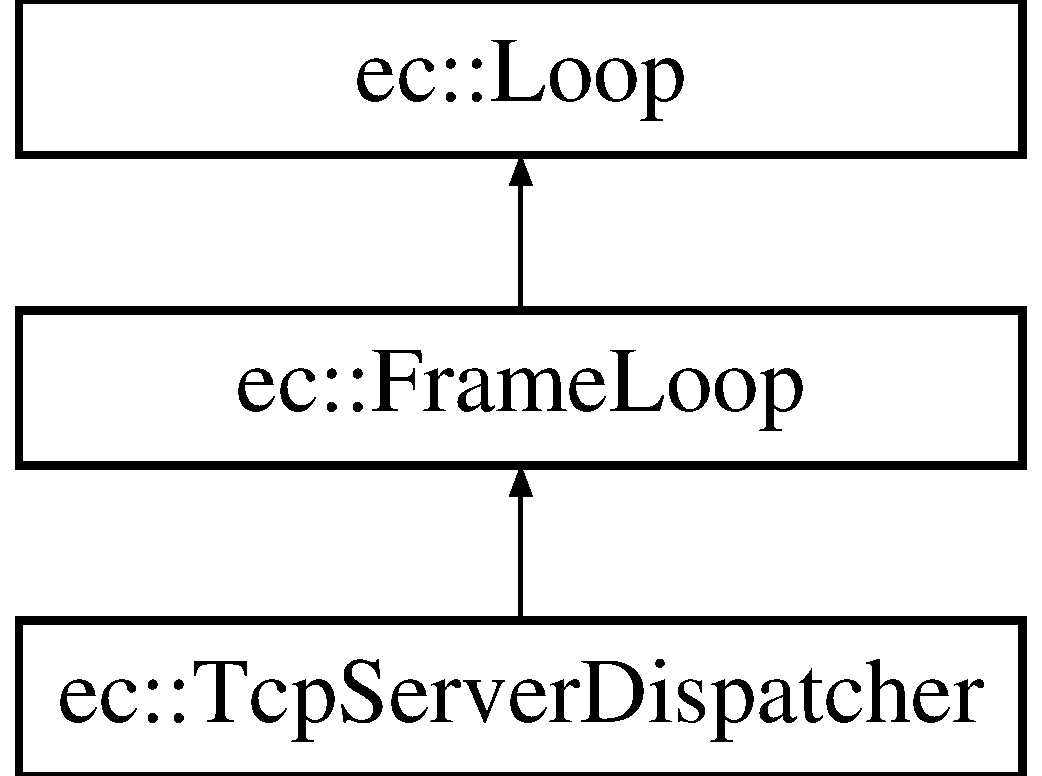
\includegraphics[height=3.000000cm]{classec_1_1FrameLoop}
\end{center}
\end{figure}
\subsection*{Public Member Functions}
\begin{DoxyCompactItemize}
\item 
void \hyperlink{classec_1_1FrameLoop_a95cd06861a99da652b30661e5238398c}{set\-Frame\-Interval} (uint32\-\_\-t interval)
\begin{DoxyCompactList}\small\item\em 设置幀时长(毫秒) \end{DoxyCompactList}\item 
\hypertarget{classec_1_1FrameLoop_a9390e3b33b561bd958a63059d67dd286}{uint64\-\_\-t \hyperlink{classec_1_1FrameLoop_a9390e3b33b561bd958a63059d67dd286}{cur\-Frame\-Round} () const }\label{classec_1_1FrameLoop_a9390e3b33b561bd958a63059d67dd286}

\begin{DoxyCompactList}\small\item\em 获取当前幀周期 \end{DoxyCompactList}\end{DoxyCompactItemize}
\subsection*{Protected Member Functions}
\begin{DoxyCompactItemize}
\item 
virtual void \hyperlink{classec_1_1FrameLoop_a8b20b1f76ed9020484a73faa80e35eb5}{on\-Before\-Loop} ()
\item 
\hypertarget{classec_1_1FrameLoop_ae4d174514e47953d75071101c49aee06}{virtual void \hyperlink{classec_1_1FrameLoop_ae4d174514e47953d75071101c49aee06}{on\-Frame} ()}\label{classec_1_1FrameLoop_ae4d174514e47953d75071101c49aee06}

\begin{DoxyCompactList}\small\item\em 每幀事件处理 \end{DoxyCompactList}\end{DoxyCompactItemize}
\subsection*{Additional Inherited Members}


\subsection{Detailed Description}
拥有幀定时器的事件循环 

由于有无限循环定时器,所以一直存在已注册的事件,不会有自动结束。默认幀时长为10毫秒 

\subsection{Member Function Documentation}
\hypertarget{classec_1_1FrameLoop_a8b20b1f76ed9020484a73faa80e35eb5}{\index{ec\-::\-Frame\-Loop@{ec\-::\-Frame\-Loop}!on\-Before\-Loop@{on\-Before\-Loop}}
\index{on\-Before\-Loop@{on\-Before\-Loop}!ec::FrameLoop@{ec\-::\-Frame\-Loop}}
\subsubsection[{on\-Before\-Loop}]{\setlength{\rightskip}{0pt plus 5cm}void ec\-::\-Frame\-Loop\-::on\-Before\-Loop (
\begin{DoxyParamCaption}
{}
\end{DoxyParamCaption}
)\hspace{0.3cm}{\ttfamily [protected]}, {\ttfamily [virtual]}}}\label{classec_1_1FrameLoop_a8b20b1f76ed9020484a73faa80e35eb5}


Reimplemented from \hyperlink{classec_1_1Loop_ab50d820e5c09ef53af2aa97a1912025a}{ec\-::\-Loop}.

\hypertarget{classec_1_1FrameLoop_a95cd06861a99da652b30661e5238398c}{\index{ec\-::\-Frame\-Loop@{ec\-::\-Frame\-Loop}!set\-Frame\-Interval@{set\-Frame\-Interval}}
\index{set\-Frame\-Interval@{set\-Frame\-Interval}!ec::FrameLoop@{ec\-::\-Frame\-Loop}}
\subsubsection[{set\-Frame\-Interval}]{\setlength{\rightskip}{0pt plus 5cm}void ec\-::\-Frame\-Loop\-::set\-Frame\-Interval (
\begin{DoxyParamCaption}
\item[{uint32\-\_\-t}]{interval}
\end{DoxyParamCaption}
)}}\label{classec_1_1FrameLoop_a95cd06861a99da652b30661e5238398c}


设置幀时长(毫秒) 

\begin{DoxyNote}{Note}
应该在启动事件循环调用
\end{DoxyNote}
没调用此函数则默认幀时长为10毫秒 
\begin{DoxyParams}{Parameters}
{\em interval} & 幀时长(毫秒),为0不会生效 \\
\hline
\end{DoxyParams}
\begin{DoxySeeAlso}{See Also}
\hyperlink{classec_1_1Loop_a5e4e5650fbd4f1716429205c84ca51fd}{Loop\-::start} 
\end{DoxySeeAlso}


The documentation for this class was generated from the following files\-:\begin{DoxyCompactItemize}
\item 
include/ec/frame\-Loop.\-h\item 
src/frame\-Loop.\-cpp\end{DoxyCompactItemize}

\hypertarget{classec_1_1HttpRequest}{\section{ec\-:\-:Http\-Request Class Reference}
\label{classec_1_1HttpRequest}\index{ec\-::\-Http\-Request@{ec\-::\-Http\-Request}}
}
\subsection*{Public Member Functions}
\begin{DoxyCompactItemize}
\item 
\hypertarget{classec_1_1HttpRequest_a7e03a8dbd2c3d2dc246161a52b6bca1a}{{\bfseries Http\-Request} (evhttp\-\_\-request $\ast$req)}\label{classec_1_1HttpRequest_a7e03a8dbd2c3d2dc246161a52b6bca1a}

\item 
\hypertarget{classec_1_1HttpRequest_ae135b819e4d9bfe1cc63575fb631b233}{const char $\ast$ {\bfseries get\-Uri} ()}\label{classec_1_1HttpRequest_ae135b819e4d9bfe1cc63575fb631b233}

\item 
\hypertarget{classec_1_1HttpRequest_add8ee458271cb64ed7ed1550c72bf227}{const char $\ast$ {\bfseries get\-Path} ()}\label{classec_1_1HttpRequest_add8ee458271cb64ed7ed1550c72bf227}

\item 
\hypertarget{classec_1_1HttpRequest_a5fba94bacedc26ea529f348a43fa3202}{const char $\ast$ {\bfseries get\-Host} ()}\label{classec_1_1HttpRequest_a5fba94bacedc26ea529f348a43fa3202}

\item 
\hypertarget{classec_1_1HttpRequest_a0bfefdeb157004726da762f1a67a248d}{uint16\-\_\-t {\bfseries get\-Port} ()}\label{classec_1_1HttpRequest_a0bfefdeb157004726da762f1a67a248d}

\item 
\hypertarget{classec_1_1HttpRequest_a4ee1d9a06f26bce0e7b666e478781885}{const char $\ast$ {\bfseries find\-Headers} (const char $\ast$key)}\label{classec_1_1HttpRequest_a4ee1d9a06f26bce0e7b666e478781885}

\item 
\hypertarget{classec_1_1HttpRequest_aa3f4b050dac178d69813cdfd2b26f454}{bool {\bfseries set\-Header} (const char $\ast$key, const char $\ast$value)}\label{classec_1_1HttpRequest_aa3f4b050dac178d69813cdfd2b26f454}

\item 
\hypertarget{classec_1_1HttpRequest_a360ff2ba5968126d03ff647b3032784e}{bool {\bfseries set\-Body} (const char $\ast$content)}\label{classec_1_1HttpRequest_a360ff2ba5968126d03ff647b3032784e}

\item 
\hypertarget{classec_1_1HttpRequest_a84830ca91e3fd9080ff06fd5a5c89f96}{bool {\bfseries set\-Chunk} (const char $\ast$content)}\label{classec_1_1HttpRequest_a84830ca91e3fd9080ff06fd5a5c89f96}

\end{DoxyCompactItemize}
\subsection*{Friends}
\begin{DoxyCompactItemize}
\item 
\hypertarget{classec_1_1HttpRequest_a7ef68af4cc3915e661d6bb0255d265d2}{class {\bfseries Http\-Server}}\label{classec_1_1HttpRequest_a7ef68af4cc3915e661d6bb0255d265d2}

\end{DoxyCompactItemize}


The documentation for this class was generated from the following files\-:\begin{DoxyCompactItemize}
\item 
include/ec/http\-Request.\-h\item 
src/http\-Request.\-cpp\end{DoxyCompactItemize}

\hypertarget{classec_1_1HttpServer}{\section{ec\-:\-:Http\-Server Class Reference}
\label{classec_1_1HttpServer}\index{ec\-::\-Http\-Server@{ec\-::\-Http\-Server}}
}
Inheritance diagram for ec\-:\-:Http\-Server\-:\begin{figure}[H]
\begin{center}
\leavevmode
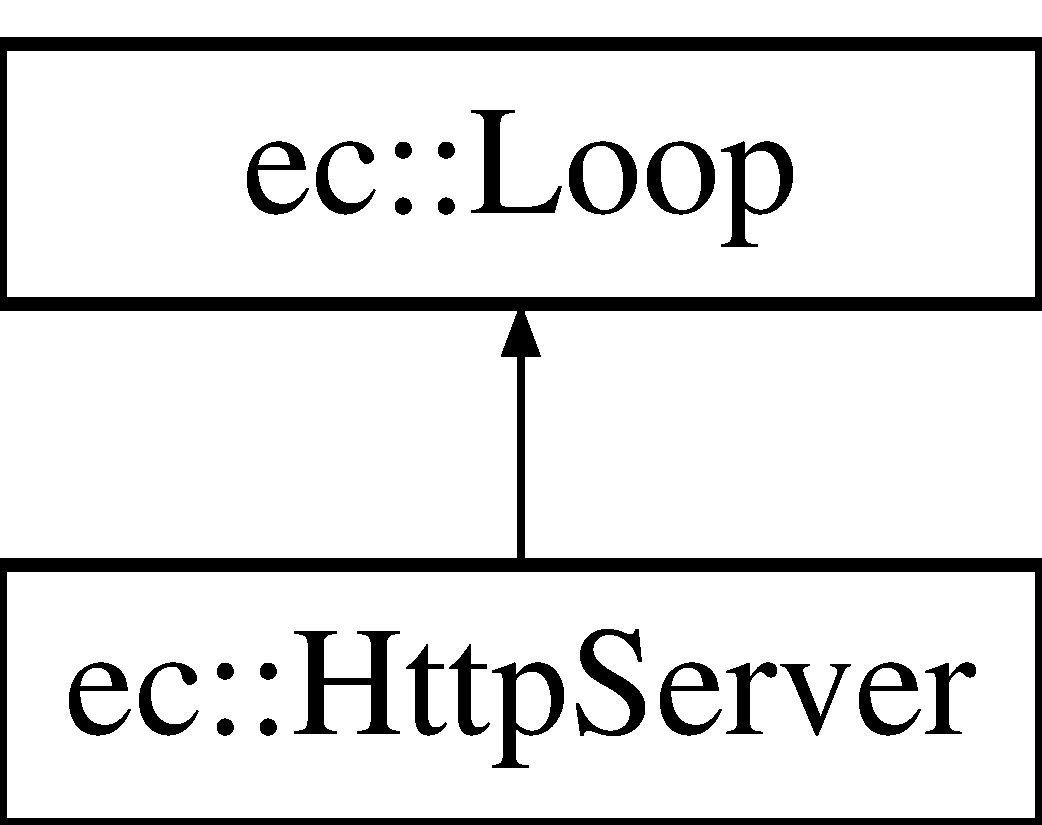
\includegraphics[height=2.000000cm]{classec_1_1HttpServer}
\end{center}
\end{figure}
\subsection*{Public Member Functions}
\begin{DoxyCompactItemize}
\item 
\hypertarget{classec_1_1HttpServer_ac56748ef31cb224abf342049f5697448}{bool {\bfseries listen} (const char $\ast$ip, uint16\-\_\-t port)}\label{classec_1_1HttpServer_ac56748ef31cb224abf342049f5697448}

\item 
\hypertarget{classec_1_1HttpServer_a0b9cf060c7a9725055e7b410cc524d56}{void {\bfseries reg\-Handler} (const char $\ast$path, ec\-::\-Http\-Handler handler)}\label{classec_1_1HttpServer_a0b9cf060c7a9725055e7b410cc524d56}

\end{DoxyCompactItemize}
\subsection*{Additional Inherited Members}


The documentation for this class was generated from the following files\-:\begin{DoxyCompactItemize}
\item 
include/ec/http\-Server.\-h\item 
src/http\-Server.\-cpp\end{DoxyCompactItemize}

\hypertarget{classec_1_1Loop}{\section{ec\-:\-:Loop Class Reference}
\label{classec_1_1Loop}\index{ec\-::\-Loop@{ec\-::\-Loop}}
}


事件循环,对event\-\_\-base的封装。  




{\ttfamily \#include $<$loop.\-h$>$}

Inheritance diagram for ec\-:\-:Loop\-:\begin{figure}[H]
\begin{center}
\leavevmode
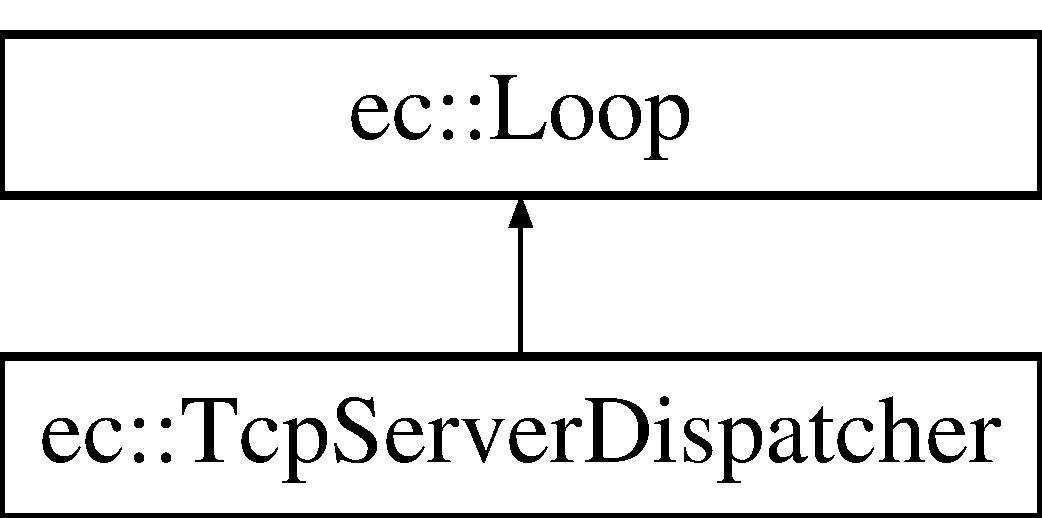
\includegraphics[height=3.000000cm]{classec_1_1Loop}
\end{center}
\end{figure}
\subsection*{Public Member Functions}
\begin{DoxyCompactItemize}
\item 
\hypertarget{classec_1_1Loop_ab104699b3b40815f32e5272e85fb01d7}{\hyperlink{classec_1_1Loop_ab104699b3b40815f32e5272e85fb01d7}{operator event\-\_\-base $\ast$} () const }\label{classec_1_1Loop_ab104699b3b40815f32e5272e85fb01d7}

\begin{DoxyCompactList}\small\item\em 转换为event\-\_\-base $\ast$指针 \end{DoxyCompactList}\item 
\hypertarget{classec_1_1Loop_af62f9eae725eda092cc52168bdcb9b53}{event\-\_\-base $\ast$ \hyperlink{classec_1_1Loop_af62f9eae725eda092cc52168bdcb9b53}{ev} () const }\label{classec_1_1Loop_af62f9eae725eda092cc52168bdcb9b53}

\begin{DoxyCompactList}\small\item\em 获取event\-\_\-base $\ast$指针 \end{DoxyCompactList}\item 
\hypertarget{classec_1_1Loop_ae60730f9a1e07de6039de8008293769a}{uint32\-\_\-t \hyperlink{classec_1_1Loop_ae60730f9a1e07de6039de8008293769a}{id} () const }\label{classec_1_1Loop_ae60730f9a1e07de6039de8008293769a}

\begin{DoxyCompactList}\small\item\em 获得自动生成的\-Id号 \end{DoxyCompactList}\item 
\hypertarget{classec_1_1Loop_a134b0eb8eaa83270eb375df11160bea5}{bool \hyperlink{classec_1_1Loop_a134b0eb8eaa83270eb375df11160bea5}{is\-Thread} () const }\label{classec_1_1Loop_a134b0eb8eaa83270eb375df11160bea5}

\begin{DoxyCompactList}\small\item\em 是否是以新线程在运行 \end{DoxyCompactList}\item 
bool \hyperlink{classec_1_1Loop_a5e4e5650fbd4f1716429205c84ca51fd}{start} (bool new\-Thread=true)
\begin{DoxyCompactList}\small\item\em 启动事件循环 \end{DoxyCompactList}\item 
void \hyperlink{classec_1_1Loop_a476329b5b1b32a9d91957fdf820ed35b}{wait} ()
\begin{DoxyCompactList}\small\item\em 等待时间循环(线程)结束 \end{DoxyCompactList}\item 
void \hyperlink{classec_1_1Loop_aa96af9467ac7882e3cea7a4dcb51005a}{stop} (bool waiting=true)
\begin{DoxyCompactList}\small\item\em 停止事件循环 \end{DoxyCompactList}\end{DoxyCompactItemize}
\subsection*{Static Public Member Functions}
\begin{DoxyCompactItemize}
\item 
static \hyperlink{classec_1_1Loop}{Loop} $\ast$ \hyperlink{classec_1_1Loop_abb797bdabdefdff5b6cc3f2b1b249747}{cur\-Loop} ()
\begin{DoxyCompactList}\small\item\em 返回当前线程的\-Loop \end{DoxyCompactList}\item 
static \hyperlink{classec_1_1Loop}{Loop} $\ast$ \hyperlink{classec_1_1Loop_a459fada2bbc382637fab88b3ce914d46}{get} (uint32\-\_\-t \hyperlink{classec_1_1Loop_ae60730f9a1e07de6039de8008293769a}{id})
\begin{DoxyCompactList}\small\item\em 根据id查找\-Loop \end{DoxyCompactList}\end{DoxyCompactItemize}
\subsection*{Protected Member Functions}
\begin{DoxyCompactItemize}
\item 
virtual bool \hyperlink{classec_1_1Loop_ab09acf916e8d3ad94cc2ceb483b1cac6}{on\-Before\-Start} ()
\begin{DoxyCompactList}\small\item\em 启动前触发 \end{DoxyCompactList}\item 
virtual void \hyperlink{classec_1_1Loop_ab50d820e5c09ef53af2aa97a1912025a}{on\-Before\-Loop} ()
\begin{DoxyCompactList}\small\item\em 事件循环运行前触发 \end{DoxyCompactList}\item 
virtual void \hyperlink{classec_1_1Loop_a9d3fec1a0d05dfdb73ceee20b6fd55b0}{on\-After\-Loop} ()
\begin{DoxyCompactList}\small\item\em 事件循环结束后触发 \end{DoxyCompactList}\item 
virtual void \hyperlink{classec_1_1Loop_aa52a4ac0232b307a08e7857748ebdd3f}{on\-After\-Stop} ()
\begin{DoxyCompactList}\small\item\em 停止后触发 \end{DoxyCompactList}\end{DoxyCompactItemize}


\subsection{Detailed Description}
事件循环,对event\-\_\-base的封装。 

类本身是线程安全的,然而事件循环只能运行在一个线程中。 如果没有已注册的事件,事件则会自动结束 

\subsection{Member Function Documentation}
\hypertarget{classec_1_1Loop_abb797bdabdefdff5b6cc3f2b1b249747}{\index{ec\-::\-Loop@{ec\-::\-Loop}!cur\-Loop@{cur\-Loop}}
\index{cur\-Loop@{cur\-Loop}!ec::Loop@{ec\-::\-Loop}}
\subsubsection[{cur\-Loop}]{\setlength{\rightskip}{0pt plus 5cm}{\bf Loop} $\ast$ ec\-::\-Loop\-::cur\-Loop (
\begin{DoxyParamCaption}
{}
\end{DoxyParamCaption}
)\hspace{0.3cm}{\ttfamily [static]}}}\label{classec_1_1Loop_abb797bdabdefdff5b6cc3f2b1b249747}


返回当前线程的\-Loop 

\begin{DoxyReturn}{Returns}
当前线程\-Loop指针,没有\-Loop则\-N\-U\-L\-L 
\end{DoxyReturn}
\hypertarget{classec_1_1Loop_a459fada2bbc382637fab88b3ce914d46}{\index{ec\-::\-Loop@{ec\-::\-Loop}!get@{get}}
\index{get@{get}!ec::Loop@{ec\-::\-Loop}}
\subsubsection[{get}]{\setlength{\rightskip}{0pt plus 5cm}{\bf Loop} $\ast$ ec\-::\-Loop\-::get (
\begin{DoxyParamCaption}
\item[{uint32\-\_\-t}]{id}
\end{DoxyParamCaption}
)\hspace{0.3cm}{\ttfamily [static]}}}\label{classec_1_1Loop_a459fada2bbc382637fab88b3ce914d46}


根据id查找\-Loop 

\begin{DoxyReturn}{Returns}
Loop指针 
\end{DoxyReturn}
\hypertarget{classec_1_1Loop_a9d3fec1a0d05dfdb73ceee20b6fd55b0}{\index{ec\-::\-Loop@{ec\-::\-Loop}!on\-After\-Loop@{on\-After\-Loop}}
\index{on\-After\-Loop@{on\-After\-Loop}!ec::Loop@{ec\-::\-Loop}}
\subsubsection[{on\-After\-Loop}]{\setlength{\rightskip}{0pt plus 5cm}void ec\-::\-Loop\-::on\-After\-Loop (
\begin{DoxyParamCaption}
{}
\end{DoxyParamCaption}
)\hspace{0.3cm}{\ttfamily [protected]}, {\ttfamily [virtual]}}}\label{classec_1_1Loop_a9d3fec1a0d05dfdb73ceee20b6fd55b0}


事件循环结束后触发 

运行在事件循环所在线程 \hypertarget{classec_1_1Loop_aa52a4ac0232b307a08e7857748ebdd3f}{\index{ec\-::\-Loop@{ec\-::\-Loop}!on\-After\-Stop@{on\-After\-Stop}}
\index{on\-After\-Stop@{on\-After\-Stop}!ec::Loop@{ec\-::\-Loop}}
\subsubsection[{on\-After\-Stop}]{\setlength{\rightskip}{0pt plus 5cm}void ec\-::\-Loop\-::on\-After\-Stop (
\begin{DoxyParamCaption}
{}
\end{DoxyParamCaption}
)\hspace{0.3cm}{\ttfamily [protected]}, {\ttfamily [virtual]}}}\label{classec_1_1Loop_aa52a4ac0232b307a08e7857748ebdd3f}


停止后触发 

运行在调用stop时所在的线程,一般实现此函数处理启动前的准备工作 \hypertarget{classec_1_1Loop_ab50d820e5c09ef53af2aa97a1912025a}{\index{ec\-::\-Loop@{ec\-::\-Loop}!on\-Before\-Loop@{on\-Before\-Loop}}
\index{on\-Before\-Loop@{on\-Before\-Loop}!ec::Loop@{ec\-::\-Loop}}
\subsubsection[{on\-Before\-Loop}]{\setlength{\rightskip}{0pt plus 5cm}void ec\-::\-Loop\-::on\-Before\-Loop (
\begin{DoxyParamCaption}
{}
\end{DoxyParamCaption}
)\hspace{0.3cm}{\ttfamily [protected]}, {\ttfamily [virtual]}}}\label{classec_1_1Loop_ab50d820e5c09ef53af2aa97a1912025a}


事件循环运行前触发 

运行在事件循环所在线程 

Reimplemented in \hyperlink{classec_1_1FrameLoop_a8b20b1f76ed9020484a73faa80e35eb5}{ec\-::\-Frame\-Loop}.

\hypertarget{classec_1_1Loop_ab09acf916e8d3ad94cc2ceb483b1cac6}{\index{ec\-::\-Loop@{ec\-::\-Loop}!on\-Before\-Start@{on\-Before\-Start}}
\index{on\-Before\-Start@{on\-Before\-Start}!ec::Loop@{ec\-::\-Loop}}
\subsubsection[{on\-Before\-Start}]{\setlength{\rightskip}{0pt plus 5cm}bool ec\-::\-Loop\-::on\-Before\-Start (
\begin{DoxyParamCaption}
{}
\end{DoxyParamCaption}
)\hspace{0.3cm}{\ttfamily [protected]}, {\ttfamily [virtual]}}}\label{classec_1_1Loop_ab09acf916e8d3ad94cc2ceb483b1cac6}


启动前触发 

运行在调用start时所在的线程,一般实现此函数处理启动前的准备工作。 \begin{DoxyReturn}{Returns}
返回false幀 
\end{DoxyReturn}
\hypertarget{classec_1_1Loop_a5e4e5650fbd4f1716429205c84ca51fd}{\index{ec\-::\-Loop@{ec\-::\-Loop}!start@{start}}
\index{start@{start}!ec::Loop@{ec\-::\-Loop}}
\subsubsection[{start}]{\setlength{\rightskip}{0pt plus 5cm}bool ec\-::\-Loop\-::start (
\begin{DoxyParamCaption}
\item[{bool}]{new\-Thread = {\ttfamily true}}
\end{DoxyParamCaption}
)}}\label{classec_1_1Loop_a5e4e5650fbd4f1716429205c84ca51fd}


启动事件循环 


\begin{DoxyParams}{Parameters}
{\em new\-Thread} & 是否启动新线程运行时间循环\\
\hline
\end{DoxyParams}
在当前线程运行会阻塞当前线程直到时间循环结束,\begin{DoxySeeAlso}{See Also}
\hyperlink{classec_1_1Loop_ab09acf916e8d3ad94cc2ceb483b1cac6}{on\-Before\-Start} 
\end{DoxySeeAlso}
\begin{DoxyReturn}{Returns}
是否成功 
\end{DoxyReturn}
\hypertarget{classec_1_1Loop_aa96af9467ac7882e3cea7a4dcb51005a}{\index{ec\-::\-Loop@{ec\-::\-Loop}!stop@{stop}}
\index{stop@{stop}!ec::Loop@{ec\-::\-Loop}}
\subsubsection[{stop}]{\setlength{\rightskip}{0pt plus 5cm}void ec\-::\-Loop\-::stop (
\begin{DoxyParamCaption}
\item[{bool}]{waiting = {\ttfamily true}}
\end{DoxyParamCaption}
)}}\label{classec_1_1Loop_aa96af9467ac7882e3cea7a4dcb51005a}


停止事件循环 

如果以新线程运行的,则会停止新线程。 
\begin{DoxyParams}{Parameters}
{\em waiting} & 是否直到运行所有激活事件的回调才退出 \\
\hline
\end{DoxyParams}
\hypertarget{classec_1_1Loop_a476329b5b1b32a9d91957fdf820ed35b}{\index{ec\-::\-Loop@{ec\-::\-Loop}!wait@{wait}}
\index{wait@{wait}!ec::Loop@{ec\-::\-Loop}}
\subsubsection[{wait}]{\setlength{\rightskip}{0pt plus 5cm}void ec\-::\-Loop\-::wait (
\begin{DoxyParamCaption}
{}
\end{DoxyParamCaption}
)}}\label{classec_1_1Loop_a476329b5b1b32a9d91957fdf820ed35b}


等待时间循环(线程)结束 

不是以新线程运行的调用此函数不会有任何效果 \begin{DoxySeeAlso}{See Also}
bool Loop\-::start\-Thread() 
\end{DoxySeeAlso}


The documentation for this class was generated from the following files\-:\begin{DoxyCompactItemize}
\item 
include/ec/loop.\-h\item 
src/loop.\-cpp\end{DoxyCompactItemize}

\hypertarget{classec_1_1TcpClient}{\section{ec\-:\-:Tcp\-Client Class Reference}
\label{classec_1_1TcpClient}\index{ec\-::\-Tcp\-Client@{ec\-::\-Tcp\-Client}}
}


客户端\-T\-C\-P连接  




{\ttfamily \#include $<$tcp\-Client.\-h$>$}

Inheritance diagram for ec\-:\-:Tcp\-Client\-:\begin{figure}[H]
\begin{center}
\leavevmode
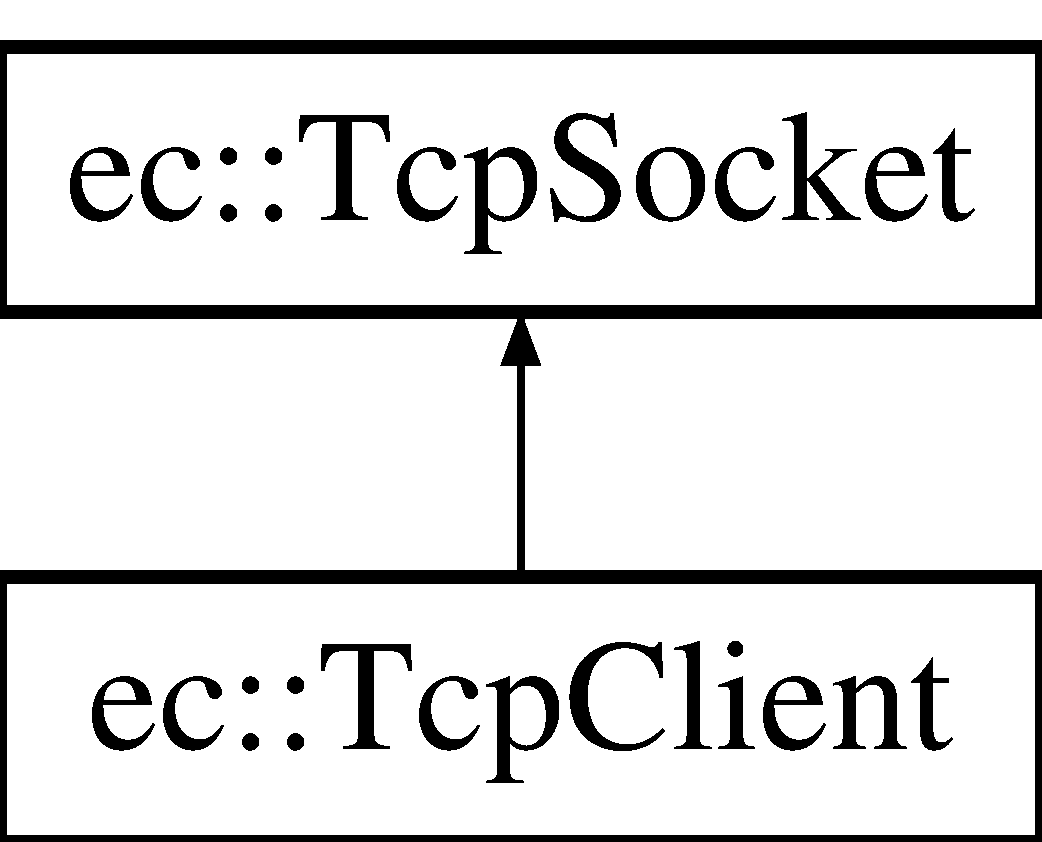
\includegraphics[height=2.000000cm]{classec_1_1TcpClient}
\end{center}
\end{figure}
\subsection*{Public Member Functions}
\begin{DoxyCompactItemize}
\item 
\hypertarget{classec_1_1TcpClient_aeddd87eefbaf668137546b0232291d8a}{{\bfseries Tcp\-Client} (const \hyperlink{classec_1_1Loop}{ec\-::\-Loop} \&loop)}\label{classec_1_1TcpClient_aeddd87eefbaf668137546b0232291d8a}

\item 
bool \hyperlink{classec_1_1TcpClient_aea5214d714c2c79d05bf0ff224b19e10}{is\-Connected} () const 
\item 
bool \hyperlink{classec_1_1TcpClient_aced7a41792c93f2b8515f2b30b265a3f}{connect} (const char $\ast$ip, uint16\-\_\-t port)
\begin{DoxyCompactList}\small\item\em 连接服务器 \end{DoxyCompactList}\end{DoxyCompactItemize}
\subsection*{Protected Member Functions}
\begin{DoxyCompactItemize}
\item 
virtual void \hyperlink{classec_1_1TcpClient_a5fb6c3ed5388a03de459b6fc233c82ea}{on\-Read} ()
\item 
virtual void \hyperlink{classec_1_1TcpClient_ad528b3c242a0f694d5a0bd1f92a614b8}{on\-Disconnected} ()
\item 
virtual void \hyperlink{classec_1_1TcpClient_adaedc4e778e2de8fca42217e305ed0da}{on\-Connected} (int error)
\begin{DoxyCompactList}\small\item\em 连接成功时处理接口 \end{DoxyCompactList}\end{DoxyCompactItemize}
\subsection*{Additional Inherited Members}


\subsection{Detailed Description}
客户端\-T\-C\-P连接 

\subsection{Member Function Documentation}
\hypertarget{classec_1_1TcpClient_aced7a41792c93f2b8515f2b30b265a3f}{\index{ec\-::\-Tcp\-Client@{ec\-::\-Tcp\-Client}!connect@{connect}}
\index{connect@{connect}!ec::TcpClient@{ec\-::\-Tcp\-Client}}
\subsubsection[{connect}]{\setlength{\rightskip}{0pt plus 5cm}bool ec\-::\-Tcp\-Client\-::connect (
\begin{DoxyParamCaption}
\item[{const char $\ast$}]{ip, }
\item[{uint16\-\_\-t}]{port}
\end{DoxyParamCaption}
)}}\label{classec_1_1TcpClient_aced7a41792c93f2b8515f2b30b265a3f}


连接服务器 


\begin{DoxyParams}{Parameters}
{\em ip} & 服务器\-I\-P地址 \\
\hline
{\em port} & 服务器监听端口 \\
\hline
\end{DoxyParams}
\begin{DoxyReturn}{Returns}
返回是否成功 
\end{DoxyReturn}
\hypertarget{classec_1_1TcpClient_aea5214d714c2c79d05bf0ff224b19e10}{\index{ec\-::\-Tcp\-Client@{ec\-::\-Tcp\-Client}!is\-Connected@{is\-Connected}}
\index{is\-Connected@{is\-Connected}!ec::TcpClient@{ec\-::\-Tcp\-Client}}
\subsubsection[{is\-Connected}]{\setlength{\rightskip}{0pt plus 5cm}bool ec\-::\-Tcp\-Client\-::is\-Connected (
\begin{DoxyParamCaption}
{}
\end{DoxyParamCaption}
) const\hspace{0.3cm}{\ttfamily [inline]}}}\label{classec_1_1TcpClient_aea5214d714c2c79d05bf0ff224b19e10}
是否已成功连接 \hypertarget{classec_1_1TcpClient_adaedc4e778e2de8fca42217e305ed0da}{\index{ec\-::\-Tcp\-Client@{ec\-::\-Tcp\-Client}!on\-Connected@{on\-Connected}}
\index{on\-Connected@{on\-Connected}!ec::TcpClient@{ec\-::\-Tcp\-Client}}
\subsubsection[{on\-Connected}]{\setlength{\rightskip}{0pt plus 5cm}virtual void ec\-::\-Tcp\-Client\-::on\-Connected (
\begin{DoxyParamCaption}
\item[{int}]{error}
\end{DoxyParamCaption}
)\hspace{0.3cm}{\ttfamily [inline]}, {\ttfamily [protected]}, {\ttfamily [virtual]}}}\label{classec_1_1TcpClient_adaedc4e778e2de8fca42217e305ed0da}


连接成功时处理接口 


\begin{DoxyParams}{Parameters}
{\em error} & 连接错误码,0表示成功 \\
\hline
\end{DoxyParams}
\hypertarget{classec_1_1TcpClient_ad528b3c242a0f694d5a0bd1f92a614b8}{\index{ec\-::\-Tcp\-Client@{ec\-::\-Tcp\-Client}!on\-Disconnected@{on\-Disconnected}}
\index{on\-Disconnected@{on\-Disconnected}!ec::TcpClient@{ec\-::\-Tcp\-Client}}
\subsubsection[{on\-Disconnected}]{\setlength{\rightskip}{0pt plus 5cm}virtual void ec\-::\-Tcp\-Client\-::on\-Disconnected (
\begin{DoxyParamCaption}
{}
\end{DoxyParamCaption}
)\hspace{0.3cm}{\ttfamily [inline]}, {\ttfamily [protected]}, {\ttfamily [virtual]}}}\label{classec_1_1TcpClient_ad528b3c242a0f694d5a0bd1f92a614b8}
连接断开时处理接口 \hypertarget{classec_1_1TcpClient_a5fb6c3ed5388a03de459b6fc233c82ea}{\index{ec\-::\-Tcp\-Client@{ec\-::\-Tcp\-Client}!on\-Read@{on\-Read}}
\index{on\-Read@{on\-Read}!ec::TcpClient@{ec\-::\-Tcp\-Client}}
\subsubsection[{on\-Read}]{\setlength{\rightskip}{0pt plus 5cm}virtual void ec\-::\-Tcp\-Client\-::on\-Read (
\begin{DoxyParamCaption}
{}
\end{DoxyParamCaption}
)\hspace{0.3cm}{\ttfamily [inline]}, {\ttfamily [protected]}, {\ttfamily [virtual]}}}\label{classec_1_1TcpClient_a5fb6c3ed5388a03de459b6fc233c82ea}
有数据可读时处理接口 

The documentation for this class was generated from the following files\-:\begin{DoxyCompactItemize}
\item 
include/ec/tcp\-Client.\-h\item 
src/tcp\-Client.\-cpp\end{DoxyCompactItemize}

\hypertarget{classec_1_1TcpServer}{\section{ec\-:\-:Tcp\-Server Class Reference}
\label{classec_1_1TcpServer}\index{ec\-::\-Tcp\-Server@{ec\-::\-Tcp\-Server}}
}


T\-C\-P服务器  




{\ttfamily \#include $<$tcp\-Server.\-h$>$}

\subsection*{Public Member Functions}
\begin{DoxyCompactItemize}
\item 
\hypertarget{classec_1_1TcpServer_acda2f66f003a4203c17886c3d70c1c77}{{\bfseries Tcp\-Server} (uint16\-\_\-t threads=0)}\label{classec_1_1TcpServer_acda2f66f003a4203c17886c3d70c1c77}

\item 
void \hyperlink{classec_1_1TcpServer_a5bb66fcd67ba08031fc65c7e2ea7220d}{set\-Threads} (uint16\-\_\-t threads)
\item 
\hyperlink{classec_1_1Loop}{ec\-::\-Loop} \& \hyperlink{classec_1_1TcpServer_a9249823c7fb037626df45335dad1c506}{get\-Loop} () const 
\item 
bool \hyperlink{classec_1_1TcpServer_a5664dc7c718dd2bd77a4f424ae49361f}{listen} (const char $\ast$ip, uint16\-\_\-t port)
\begin{DoxyCompactList}\small\item\em 监听 \end{DoxyCompactList}\item 
void \hyperlink{classec_1_1TcpServer_ad7312d86be0f2ad13d24de79c77298c3}{stop} ()
\item 
void \hyperlink{classec_1_1TcpServer_ad37edaf6e644d00b80c90610f4ca4ad5}{wait} ()
\end{DoxyCompactItemize}
\subsection*{Protected Member Functions}
\begin{DoxyCompactItemize}
\item 
virtual void \hyperlink{classec_1_1TcpServer_aa70b8c0ff54b76b78492bd02c1396d40}{on\-Listen\-Error} ()
\item 
virtual void \hyperlink{classec_1_1TcpServer_afd151d6640eda1e7de6934292d0ce045}{on\-Session\-Read} (\hyperlink{classec_1_1TcpSession}{ec\-::\-Tcp\-Session} $\ast$session)
\item 
virtual void \hyperlink{classec_1_1TcpServer_a6c6e9583952b194f6510b1d67c960682}{on\-Session\-Disconnected} (\hyperlink{classec_1_1TcpSession}{ec\-::\-Tcp\-Session} $\ast$session)
\item 
virtual void \hyperlink{classec_1_1TcpServer_a3fb6ace162987df6f7375ef08346f8f8}{on\-New\-Session} (\hyperlink{classec_1_1TcpSession}{ec\-::\-Tcp\-Session} $\ast$session)
\end{DoxyCompactItemize}
\subsection*{Friends}
\begin{DoxyCompactItemize}
\item 
\hypertarget{classec_1_1TcpServer_ad821fb654cf0b89cb6245fa831ec471c}{class {\bfseries Tcp\-Session}}\label{classec_1_1TcpServer_ad821fb654cf0b89cb6245fa831ec471c}

\item 
\hypertarget{classec_1_1TcpServer_aacbf5c26d9d3dde89d5ebccceb97ad3f}{class {\bfseries Tcp\-Server\-Dispatcher}}\label{classec_1_1TcpServer_aacbf5c26d9d3dde89d5ebccceb97ad3f}

\end{DoxyCompactItemize}


\subsection{Detailed Description}
T\-C\-P服务器 

其包含了一个监听线程和多个\-I\-O线程 

\subsection{Member Function Documentation}
\hypertarget{classec_1_1TcpServer_a9249823c7fb037626df45335dad1c506}{\index{ec\-::\-Tcp\-Server@{ec\-::\-Tcp\-Server}!get\-Loop@{get\-Loop}}
\index{get\-Loop@{get\-Loop}!ec::TcpServer@{ec\-::\-Tcp\-Server}}
\subsubsection[{get\-Loop}]{\setlength{\rightskip}{0pt plus 5cm}{\bf ec\-::\-Loop}\& ec\-::\-Tcp\-Server\-::get\-Loop (
\begin{DoxyParamCaption}
{}
\end{DoxyParamCaption}
) const\hspace{0.3cm}{\ttfamily [inline]}}}\label{classec_1_1TcpServer_a9249823c7fb037626df45335dad1c506}
获取\-Loop包含的\-Loop对象引用 \hypertarget{classec_1_1TcpServer_a5664dc7c718dd2bd77a4f424ae49361f}{\index{ec\-::\-Tcp\-Server@{ec\-::\-Tcp\-Server}!listen@{listen}}
\index{listen@{listen}!ec::TcpServer@{ec\-::\-Tcp\-Server}}
\subsubsection[{listen}]{\setlength{\rightskip}{0pt plus 5cm}bool ec\-::\-Tcp\-Server\-::listen (
\begin{DoxyParamCaption}
\item[{const char $\ast$}]{ip, }
\item[{uint16\-\_\-t}]{port}
\end{DoxyParamCaption}
)}}\label{classec_1_1TcpServer_a5664dc7c718dd2bd77a4f424ae49361f}


监听 


\begin{DoxyParams}{Parameters}
{\em ip} & 服务器\-I\-P地址 \\
\hline
{\em port} & 服务器监听端口 \\
\hline
\end{DoxyParams}
\begin{DoxyReturn}{Returns}
返回是否成功 
\end{DoxyReturn}
\hypertarget{classec_1_1TcpServer_aa70b8c0ff54b76b78492bd02c1396d40}{\index{ec\-::\-Tcp\-Server@{ec\-::\-Tcp\-Server}!on\-Listen\-Error@{on\-Listen\-Error}}
\index{on\-Listen\-Error@{on\-Listen\-Error}!ec::TcpServer@{ec\-::\-Tcp\-Server}}
\subsubsection[{on\-Listen\-Error}]{\setlength{\rightskip}{0pt plus 5cm}virtual void ec\-::\-Tcp\-Server\-::on\-Listen\-Error (
\begin{DoxyParamCaption}
{}
\end{DoxyParamCaption}
)\hspace{0.3cm}{\ttfamily [inline]}, {\ttfamily [protected]}, {\ttfamily [virtual]}}}\label{classec_1_1TcpServer_aa70b8c0ff54b76b78492bd02c1396d40}
监听失败时处理接口 \hypertarget{classec_1_1TcpServer_a3fb6ace162987df6f7375ef08346f8f8}{\index{ec\-::\-Tcp\-Server@{ec\-::\-Tcp\-Server}!on\-New\-Session@{on\-New\-Session}}
\index{on\-New\-Session@{on\-New\-Session}!ec::TcpServer@{ec\-::\-Tcp\-Server}}
\subsubsection[{on\-New\-Session}]{\setlength{\rightskip}{0pt plus 5cm}virtual void ec\-::\-Tcp\-Server\-::on\-New\-Session (
\begin{DoxyParamCaption}
\item[{{\bf ec\-::\-Tcp\-Session} $\ast$}]{session}
\end{DoxyParamCaption}
)\hspace{0.3cm}{\ttfamily [inline]}, {\ttfamily [protected]}, {\ttfamily [virtual]}}}\label{classec_1_1TcpServer_a3fb6ace162987df6f7375ef08346f8f8}
有新连接时处理接口 \hypertarget{classec_1_1TcpServer_a6c6e9583952b194f6510b1d67c960682}{\index{ec\-::\-Tcp\-Server@{ec\-::\-Tcp\-Server}!on\-Session\-Disconnected@{on\-Session\-Disconnected}}
\index{on\-Session\-Disconnected@{on\-Session\-Disconnected}!ec::TcpServer@{ec\-::\-Tcp\-Server}}
\subsubsection[{on\-Session\-Disconnected}]{\setlength{\rightskip}{0pt plus 5cm}virtual void ec\-::\-Tcp\-Server\-::on\-Session\-Disconnected (
\begin{DoxyParamCaption}
\item[{{\bf ec\-::\-Tcp\-Session} $\ast$}]{session}
\end{DoxyParamCaption}
)\hspace{0.3cm}{\ttfamily [inline]}, {\ttfamily [protected]}, {\ttfamily [virtual]}}}\label{classec_1_1TcpServer_a6c6e9583952b194f6510b1d67c960682}
连接断开时处理接口 \hypertarget{classec_1_1TcpServer_afd151d6640eda1e7de6934292d0ce045}{\index{ec\-::\-Tcp\-Server@{ec\-::\-Tcp\-Server}!on\-Session\-Read@{on\-Session\-Read}}
\index{on\-Session\-Read@{on\-Session\-Read}!ec::TcpServer@{ec\-::\-Tcp\-Server}}
\subsubsection[{on\-Session\-Read}]{\setlength{\rightskip}{0pt plus 5cm}virtual void ec\-::\-Tcp\-Server\-::on\-Session\-Read (
\begin{DoxyParamCaption}
\item[{{\bf ec\-::\-Tcp\-Session} $\ast$}]{session}
\end{DoxyParamCaption}
)\hspace{0.3cm}{\ttfamily [inline]}, {\ttfamily [protected]}, {\ttfamily [virtual]}}}\label{classec_1_1TcpServer_afd151d6640eda1e7de6934292d0ce045}
连接有数据可读时处理接口 \hypertarget{classec_1_1TcpServer_a5bb66fcd67ba08031fc65c7e2ea7220d}{\index{ec\-::\-Tcp\-Server@{ec\-::\-Tcp\-Server}!set\-Threads@{set\-Threads}}
\index{set\-Threads@{set\-Threads}!ec::TcpServer@{ec\-::\-Tcp\-Server}}
\subsubsection[{set\-Threads}]{\setlength{\rightskip}{0pt plus 5cm}void ec\-::\-Tcp\-Server\-::set\-Threads (
\begin{DoxyParamCaption}
\item[{uint16\-\_\-t}]{threads}
\end{DoxyParamCaption}
)}}\label{classec_1_1TcpServer_a5bb66fcd67ba08031fc65c7e2ea7220d}
设置\-I\-O线程数量,需在监听之前调用 \hypertarget{classec_1_1TcpServer_ad7312d86be0f2ad13d24de79c77298c3}{\index{ec\-::\-Tcp\-Server@{ec\-::\-Tcp\-Server}!stop@{stop}}
\index{stop@{stop}!ec::TcpServer@{ec\-::\-Tcp\-Server}}
\subsubsection[{stop}]{\setlength{\rightskip}{0pt plus 5cm}void ec\-::\-Tcp\-Server\-::stop (
\begin{DoxyParamCaption}
{}
\end{DoxyParamCaption}
)}}\label{classec_1_1TcpServer_ad7312d86be0f2ad13d24de79c77298c3}
停止 \hypertarget{classec_1_1TcpServer_ad37edaf6e644d00b80c90610f4ca4ad5}{\index{ec\-::\-Tcp\-Server@{ec\-::\-Tcp\-Server}!wait@{wait}}
\index{wait@{wait}!ec::TcpServer@{ec\-::\-Tcp\-Server}}
\subsubsection[{wait}]{\setlength{\rightskip}{0pt plus 5cm}void ec\-::\-Tcp\-Server\-::wait (
\begin{DoxyParamCaption}
{}
\end{DoxyParamCaption}
)}}\label{classec_1_1TcpServer_ad37edaf6e644d00b80c90610f4ca4ad5}
等待所有线程结束 

The documentation for this class was generated from the following files\-:\begin{DoxyCompactItemize}
\item 
include/ec/tcp\-Server.\-h\item 
src/tcp\-Server.\-cpp\end{DoxyCompactItemize}

\hypertarget{classec_1_1TcpServerDispatcher}{\section{ec\-:\-:Tcp\-Server\-Dispatcher Class Reference}
\label{classec_1_1TcpServerDispatcher}\index{ec\-::\-Tcp\-Server\-Dispatcher@{ec\-::\-Tcp\-Server\-Dispatcher}}
}


T\-C\-P服务器会话调度管理器  




{\ttfamily \#include $<$tcp\-Server\-Dispatcher.\-h$>$}

Inheritance diagram for ec\-:\-:Tcp\-Server\-Dispatcher\-:\begin{figure}[H]
\begin{center}
\leavevmode
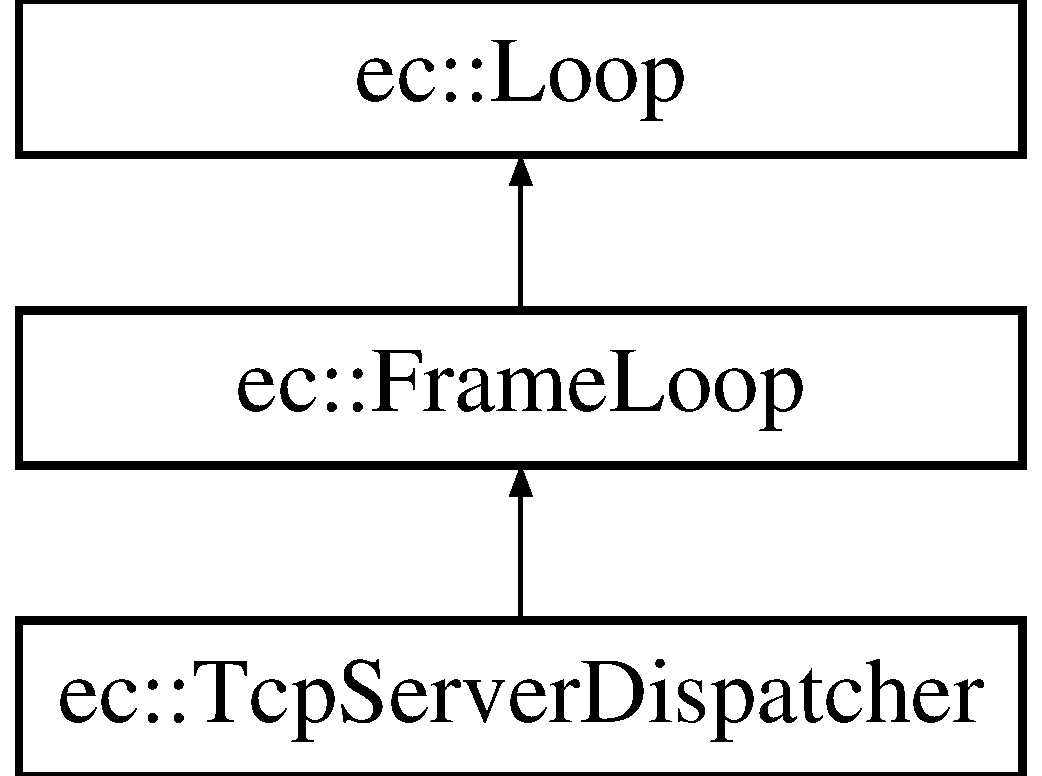
\includegraphics[height=2.000000cm]{classec_1_1TcpServerDispatcher}
\end{center}
\end{figure}
\subsection*{Classes}
\begin{DoxyCompactItemize}
\item 
struct \hyperlink{structec_1_1TcpServerDispatcher_1_1NewSessionData}{New\-Session\-Data}
\end{DoxyCompactItemize}
\subsection*{Public Member Functions}
\begin{DoxyCompactItemize}
\item 
\hypertarget{classec_1_1TcpServerDispatcher_a0fcac28c897fdccaabf54ddd1f718caa}{{\bfseries Tcp\-Server\-Dispatcher} (\hyperlink{classec_1_1TcpServer}{Tcp\-Server} $\ast$server)}\label{classec_1_1TcpServerDispatcher_a0fcac28c897fdccaabf54ddd1f718caa}

\item 
\hypertarget{classec_1_1TcpServerDispatcher_a039333f36785f4405a0fac6661a1398a}{\hyperlink{classec_1_1TcpServer}{ec\-::\-Tcp\-Server} $\ast$ {\bfseries get\-Server} () const }\label{classec_1_1TcpServerDispatcher_a039333f36785f4405a0fac6661a1398a}

\item 
\hypertarget{classec_1_1TcpServerDispatcher_acdc755e605191a51778baddf03b425cd}{ec\-::\-Tcp\-Session\-Ptr {\bfseries get\-Session} (ec\-::\-Session\-Id id)}\label{classec_1_1TcpServerDispatcher_acdc755e605191a51778baddf03b425cd}

\end{DoxyCompactItemize}
\subsection*{Protected Member Functions}
\begin{DoxyCompactItemize}
\item 
\hypertarget{classec_1_1TcpServerDispatcher_a5dbcd5063ae16237b7228f87832832db}{virtual void \hyperlink{classec_1_1TcpServerDispatcher_a5dbcd5063ae16237b7228f87832832db}{on\-Post} (\hyperlink{classec_1_1Data}{ec\-::\-Data} \&data)}\label{classec_1_1TcpServerDispatcher_a5dbcd5063ae16237b7228f87832832db}

\begin{DoxyCompactList}\small\item\em 继承此接口处理异步数据 \end{DoxyCompactList}\end{DoxyCompactItemize}
\subsection*{Friends}
\begin{DoxyCompactItemize}
\item 
\hypertarget{classec_1_1TcpServerDispatcher_ad821fb654cf0b89cb6245fa831ec471c}{class {\bfseries Tcp\-Session}}\label{classec_1_1TcpServerDispatcher_ad821fb654cf0b89cb6245fa831ec471c}

\end{DoxyCompactItemize}
\subsection*{Additional Inherited Members}


\subsection{Detailed Description}
T\-C\-P服务器会话调度管理器 

Tcp\-Server负责监听连接,然后分配给\-Tcp\-Server\-Dispatcher管理 \begin{DoxySeeAlso}{See Also}
\hyperlink{classec_1_1TcpServer}{ec\-::\-Tcp\-Server} 
\end{DoxySeeAlso}


The documentation for this class was generated from the following files\-:\begin{DoxyCompactItemize}
\item 
include/ec/tcp\-Server\-Dispatcher.\-h\item 
src/tcp\-Server\-Dispatcher.\-cpp\end{DoxyCompactItemize}

\hypertarget{classec_1_1TcpSession}{\section{ec\-:\-:Tcp\-Session Class Reference}
\label{classec_1_1TcpSession}\index{ec\-::\-Tcp\-Session@{ec\-::\-Tcp\-Session}}
}


服务端\-T\-C\-P连接  




{\ttfamily \#include $<$tcp\-Session.\-h$>$}

Inheritance diagram for ec\-:\-:Tcp\-Session\-:\begin{figure}[H]
\begin{center}
\leavevmode
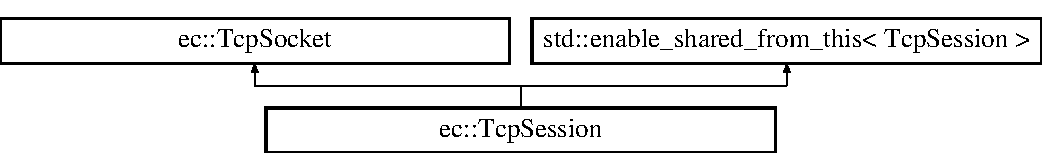
\includegraphics[height=2.000000cm]{classec_1_1TcpSession}
\end{center}
\end{figure}
\subsection*{Public Member Functions}
\begin{DoxyCompactItemize}
\item 
\hypertarget{classec_1_1TcpSession_abfc38f6a02ca6dfce9474a9a1b9dc52d}{{\bfseries Tcp\-Session} (\hyperlink{classec_1_1TcpServerDispatcher}{ec\-::\-Tcp\-Server\-Dispatcher} $\ast$dispatcher, ec\-::\-Session\-Id id)}\label{classec_1_1TcpSession_abfc38f6a02ca6dfce9474a9a1b9dc52d}

\item 
\hyperlink{classec_1_1TcpServerDispatcher}{ec\-::\-Tcp\-Server\-Dispatcher} $\ast$ \hyperlink{classec_1_1TcpSession_af4ff735c6120233feccc3a1ca29bbf04}{get\-Dispatcher} () const 
\item 
ec\-::\-Session\-Id \hyperlink{classec_1_1TcpSession_af00a92d50517f1f26cbe8d23d07452be}{get\-Id} () const 
\item 
void \hyperlink{classec_1_1TcpSession_a098cb072909ba5452f47397a787311f4}{attach} (ec\-::\-Socket\-Fd sock)
\end{DoxyCompactItemize}
\subsection*{Additional Inherited Members}


\subsection{Detailed Description}
服务端\-T\-C\-P连接 

\subsection{Member Function Documentation}
\hypertarget{classec_1_1TcpSession_a098cb072909ba5452f47397a787311f4}{\index{ec\-::\-Tcp\-Session@{ec\-::\-Tcp\-Session}!attach@{attach}}
\index{attach@{attach}!ec::TcpSession@{ec\-::\-Tcp\-Session}}
\subsubsection[{attach}]{\setlength{\rightskip}{0pt plus 5cm}void ec\-::\-Tcp\-Session\-::attach (
\begin{DoxyParamCaption}
\item[{ec\-::\-Socket\-Fd}]{sock}
\end{DoxyParamCaption}
)}}\label{classec_1_1TcpSession_a098cb072909ba5452f47397a787311f4}
关联到某socket \hypertarget{classec_1_1TcpSession_af4ff735c6120233feccc3a1ca29bbf04}{\index{ec\-::\-Tcp\-Session@{ec\-::\-Tcp\-Session}!get\-Dispatcher@{get\-Dispatcher}}
\index{get\-Dispatcher@{get\-Dispatcher}!ec::TcpSession@{ec\-::\-Tcp\-Session}}
\subsubsection[{get\-Dispatcher}]{\setlength{\rightskip}{0pt plus 5cm}{\bf ec\-::\-Tcp\-Server\-Dispatcher}$\ast$ ec\-::\-Tcp\-Session\-::get\-Dispatcher (
\begin{DoxyParamCaption}
{}
\end{DoxyParamCaption}
) const\hspace{0.3cm}{\ttfamily [inline]}}}\label{classec_1_1TcpSession_af4ff735c6120233feccc3a1ca29bbf04}
获取管理此连接的调度器 \hypertarget{classec_1_1TcpSession_af00a92d50517f1f26cbe8d23d07452be}{\index{ec\-::\-Tcp\-Session@{ec\-::\-Tcp\-Session}!get\-Id@{get\-Id}}
\index{get\-Id@{get\-Id}!ec::TcpSession@{ec\-::\-Tcp\-Session}}
\subsubsection[{get\-Id}]{\setlength{\rightskip}{0pt plus 5cm}ec\-::\-Session\-Id ec\-::\-Tcp\-Session\-::get\-Id (
\begin{DoxyParamCaption}
{}
\end{DoxyParamCaption}
) const\hspace{0.3cm}{\ttfamily [inline]}}}\label{classec_1_1TcpSession_af00a92d50517f1f26cbe8d23d07452be}
获取唯一会话id 

The documentation for this class was generated from the following files\-:\begin{DoxyCompactItemize}
\item 
include/ec/tcp\-Session.\-h\item 
src/tcp\-Session.\-cpp\end{DoxyCompactItemize}

\hypertarget{classec_1_1TcpSocket}{\section{ec\-:\-:Tcp\-Socket Class Reference}
\label{classec_1_1TcpSocket}\index{ec\-::\-Tcp\-Socket@{ec\-::\-Tcp\-Socket}}
}


T\-C\-P连接基类  




{\ttfamily \#include $<$tcp\-Socket.\-h$>$}

Inheritance diagram for ec\-:\-:Tcp\-Socket\-:\begin{figure}[H]
\begin{center}
\leavevmode
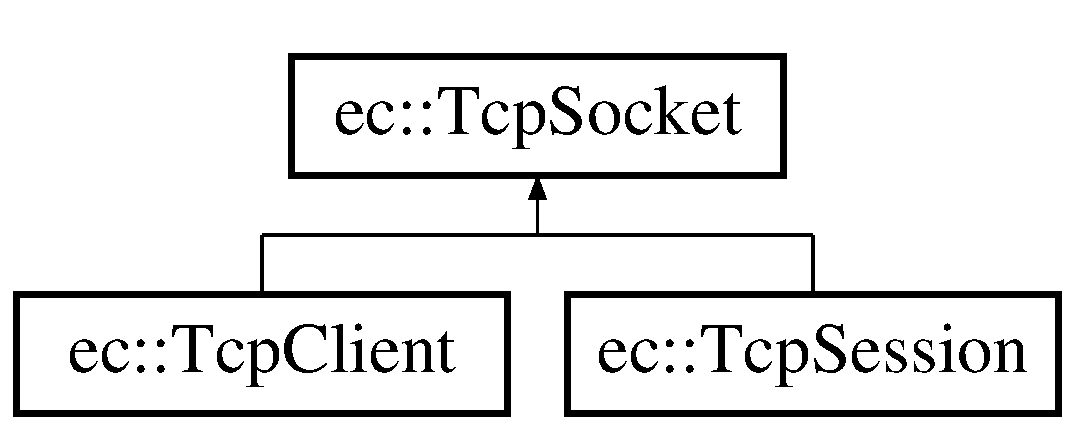
\includegraphics[height=2.000000cm]{classec_1_1TcpSocket}
\end{center}
\end{figure}
\subsection*{Public Member Functions}
\begin{DoxyCompactItemize}
\item 
bool \hyperlink{classec_1_1TcpSocket_a75615a2cb729bf1e11f7bf9414dedb6e}{is\-Inited} () const 
\item 
Socket\-Fd \hyperlink{classec_1_1TcpSocket_a5612ba87be272ed6dcc50d3dd097070c}{get\-Socket} () const 
\item 
void \hyperlink{classec_1_1TcpSocket_ac2b55cbb75000a218b3c1d83c1365611}{get\-Addr} (struct sockaddr\-\_\-in $\ast$dest, uint32\-\_\-t size) const 
\item 
bool \hyperlink{classec_1_1TcpSocket_af9e2fdbb732d93537e2867eeebc34ab2}{send} (const char $\ast$data, uint32\-\_\-t size)
\begin{DoxyCompactList}\small\item\em 发送数据 \end{DoxyCompactList}\item 
void \hyperlink{classec_1_1TcpSocket_aac8cfc7de1d70f850ec304a40ef814a6}{close} (bool waiting=true)
\begin{DoxyCompactList}\small\item\em 关闭连接 \end{DoxyCompactList}\item 
uint32\-\_\-t \hyperlink{classec_1_1TcpSocket_a73baa70135fad8207968cfc2c7c6fe2a}{get\-Input\-Buffer\-Length} () const 
\item 
const uint8\-\_\-t $\ast$ \hyperlink{classec_1_1TcpSocket_a50a9ce465e5c0e0c20fe63f99cc294af}{view\-Input\-Buffer} (uint32\-\_\-t size) const 
\item 
bool \hyperlink{classec_1_1TcpSocket_a64a402951553c83c1ba6be46fcf642d0}{read\-Input\-Buffer} (uint8\-\_\-t $\ast$dest, uint32\-\_\-t size)
\item 
void \hyperlink{classec_1_1TcpSocket_a55626e2cba2d193b4aa04ee0fc8a197e}{clear\-Input\-Buffer} ()
\end{DoxyCompactItemize}
\subsection*{Protected Member Functions}
\begin{DoxyCompactItemize}
\item 
\hypertarget{classec_1_1TcpSocket_ae5053578ebd24aac2aaf6e7a697a71d6}{void {\bfseries check\-Closing} ()}\label{classec_1_1TcpSocket_ae5053578ebd24aac2aaf6e7a697a71d6}

\end{DoxyCompactItemize}
\subsection*{Protected Attributes}
\begin{DoxyCompactItemize}
\item 
\hypertarget{classec_1_1TcpSocket_a13725375b3f583451cc71e907ca9e919}{struct bufferevent $\ast$ {\bfseries \-\_\-bev}}\label{classec_1_1TcpSocket_a13725375b3f583451cc71e907ca9e919}

\end{DoxyCompactItemize}


\subsection{Detailed Description}
T\-C\-P连接基类 

\subsection{Member Function Documentation}
\hypertarget{classec_1_1TcpSocket_a55626e2cba2d193b4aa04ee0fc8a197e}{\index{ec\-::\-Tcp\-Socket@{ec\-::\-Tcp\-Socket}!clear\-Input\-Buffer@{clear\-Input\-Buffer}}
\index{clear\-Input\-Buffer@{clear\-Input\-Buffer}!ec::TcpSocket@{ec\-::\-Tcp\-Socket}}
\subsubsection[{clear\-Input\-Buffer}]{\setlength{\rightskip}{0pt plus 5cm}void ec\-::\-Tcp\-Socket\-::clear\-Input\-Buffer (
\begin{DoxyParamCaption}
{}
\end{DoxyParamCaption}
)}}\label{classec_1_1TcpSocket_a55626e2cba2d193b4aa04ee0fc8a197e}
清空收数据缓冲区 \hypertarget{classec_1_1TcpSocket_aac8cfc7de1d70f850ec304a40ef814a6}{\index{ec\-::\-Tcp\-Socket@{ec\-::\-Tcp\-Socket}!close@{close}}
\index{close@{close}!ec::TcpSocket@{ec\-::\-Tcp\-Socket}}
\subsubsection[{close}]{\setlength{\rightskip}{0pt plus 5cm}void ec\-::\-Tcp\-Socket\-::close (
\begin{DoxyParamCaption}
\item[{bool}]{waiting = {\ttfamily true}}
\end{DoxyParamCaption}
)}}\label{classec_1_1TcpSocket_aac8cfc7de1d70f850ec304a40ef814a6}


关闭连接 


\begin{DoxyParams}{Parameters}
{\em waiting} & 是否等待数据发送完再关闭 \\
\hline
\end{DoxyParams}
\hypertarget{classec_1_1TcpSocket_ac2b55cbb75000a218b3c1d83c1365611}{\index{ec\-::\-Tcp\-Socket@{ec\-::\-Tcp\-Socket}!get\-Addr@{get\-Addr}}
\index{get\-Addr@{get\-Addr}!ec::TcpSocket@{ec\-::\-Tcp\-Socket}}
\subsubsection[{get\-Addr}]{\setlength{\rightskip}{0pt plus 5cm}void ec\-::\-Tcp\-Socket\-::get\-Addr (
\begin{DoxyParamCaption}
\item[{struct sockaddr\-\_\-in $\ast$}]{dest, }
\item[{uint32\-\_\-t}]{size}
\end{DoxyParamCaption}
) const}}\label{classec_1_1TcpSocket_ac2b55cbb75000a218b3c1d83c1365611}
获取连接地址 \hypertarget{classec_1_1TcpSocket_a73baa70135fad8207968cfc2c7c6fe2a}{\index{ec\-::\-Tcp\-Socket@{ec\-::\-Tcp\-Socket}!get\-Input\-Buffer\-Length@{get\-Input\-Buffer\-Length}}
\index{get\-Input\-Buffer\-Length@{get\-Input\-Buffer\-Length}!ec::TcpSocket@{ec\-::\-Tcp\-Socket}}
\subsubsection[{get\-Input\-Buffer\-Length}]{\setlength{\rightskip}{0pt plus 5cm}uint32\-\_\-t ec\-::\-Tcp\-Socket\-::get\-Input\-Buffer\-Length (
\begin{DoxyParamCaption}
{}
\end{DoxyParamCaption}
) const}}\label{classec_1_1TcpSocket_a73baa70135fad8207968cfc2c7c6fe2a}
获取收数据缓冲区数据长度 \hypertarget{classec_1_1TcpSocket_a5612ba87be272ed6dcc50d3dd097070c}{\index{ec\-::\-Tcp\-Socket@{ec\-::\-Tcp\-Socket}!get\-Socket@{get\-Socket}}
\index{get\-Socket@{get\-Socket}!ec::TcpSocket@{ec\-::\-Tcp\-Socket}}
\subsubsection[{get\-Socket}]{\setlength{\rightskip}{0pt plus 5cm}Socket\-Fd ec\-::\-Tcp\-Socket\-::get\-Socket (
\begin{DoxyParamCaption}
{}
\end{DoxyParamCaption}
) const}}\label{classec_1_1TcpSocket_a5612ba87be272ed6dcc50d3dd097070c}
获取socket \hypertarget{classec_1_1TcpSocket_a75615a2cb729bf1e11f7bf9414dedb6e}{\index{ec\-::\-Tcp\-Socket@{ec\-::\-Tcp\-Socket}!is\-Inited@{is\-Inited}}
\index{is\-Inited@{is\-Inited}!ec::TcpSocket@{ec\-::\-Tcp\-Socket}}
\subsubsection[{is\-Inited}]{\setlength{\rightskip}{0pt plus 5cm}bool ec\-::\-Tcp\-Socket\-::is\-Inited (
\begin{DoxyParamCaption}
{}
\end{DoxyParamCaption}
) const\hspace{0.3cm}{\ttfamily [inline]}}}\label{classec_1_1TcpSocket_a75615a2cb729bf1e11f7bf9414dedb6e}
是否已初始化 \hypertarget{classec_1_1TcpSocket_a64a402951553c83c1ba6be46fcf642d0}{\index{ec\-::\-Tcp\-Socket@{ec\-::\-Tcp\-Socket}!read\-Input\-Buffer@{read\-Input\-Buffer}}
\index{read\-Input\-Buffer@{read\-Input\-Buffer}!ec::TcpSocket@{ec\-::\-Tcp\-Socket}}
\subsubsection[{read\-Input\-Buffer}]{\setlength{\rightskip}{0pt plus 5cm}bool ec\-::\-Tcp\-Socket\-::read\-Input\-Buffer (
\begin{DoxyParamCaption}
\item[{uint8\-\_\-t $\ast$}]{dest, }
\item[{uint32\-\_\-t}]{size}
\end{DoxyParamCaption}
)}}\label{classec_1_1TcpSocket_a64a402951553c83c1ba6be46fcf642d0}
读取收数据缓冲区 \hypertarget{classec_1_1TcpSocket_af9e2fdbb732d93537e2867eeebc34ab2}{\index{ec\-::\-Tcp\-Socket@{ec\-::\-Tcp\-Socket}!send@{send}}
\index{send@{send}!ec::TcpSocket@{ec\-::\-Tcp\-Socket}}
\subsubsection[{send}]{\setlength{\rightskip}{0pt plus 5cm}bool ec\-::\-Tcp\-Socket\-::send (
\begin{DoxyParamCaption}
\item[{const char $\ast$}]{data, }
\item[{uint32\-\_\-t}]{size}
\end{DoxyParamCaption}
)}}\label{classec_1_1TcpSocket_af9e2fdbb732d93537e2867eeebc34ab2}


发送数据 


\begin{DoxyParams}{Parameters}
{\em data} & 数据地址 \\
\hline
{\em size} & 数据字节大小 \\
\hline
\end{DoxyParams}
\begin{DoxyReturn}{Returns}
返回是否成功 
\end{DoxyReturn}
\hypertarget{classec_1_1TcpSocket_a50a9ce465e5c0e0c20fe63f99cc294af}{\index{ec\-::\-Tcp\-Socket@{ec\-::\-Tcp\-Socket}!view\-Input\-Buffer@{view\-Input\-Buffer}}
\index{view\-Input\-Buffer@{view\-Input\-Buffer}!ec::TcpSocket@{ec\-::\-Tcp\-Socket}}
\subsubsection[{view\-Input\-Buffer}]{\setlength{\rightskip}{0pt plus 5cm}const uint8\-\_\-t $\ast$ ec\-::\-Tcp\-Socket\-::view\-Input\-Buffer (
\begin{DoxyParamCaption}
\item[{uint32\-\_\-t}]{size}
\end{DoxyParamCaption}
) const}}\label{classec_1_1TcpSocket_a50a9ce465e5c0e0c20fe63f99cc294af}
查看收数据缓冲区 

The documentation for this class was generated from the following files\-:\begin{DoxyCompactItemize}
\item 
include/ec/tcp\-Socket.\-h\item 
src/tcp\-Socket.\-cpp\end{DoxyCompactItemize}

\hypertarget{classec_1_1Time}{\section{ec\-:\-:Time Class Reference}
\label{classec_1_1Time}\index{ec\-::\-Time@{ec\-::\-Time}}
}


时间类  




{\ttfamily \#include $<$date.\-h$>$}

\subsection*{Public Types}
\begin{DoxyCompactItemize}
\item 
enum \hyperlink{classec_1_1Time_a5a62816a9c7f2df3ca66f54d1544ea46}{Period\-Type} \{ \\*
{\bfseries k\-Period\-None} = 0, 
\hyperlink{classec_1_1Time_a5a62816a9c7f2df3ca66f54d1544ea46a3077b99141eef7503633f22c0424bc8d}{k\-Period\-Minute}, 
\hyperlink{classec_1_1Time_a5a62816a9c7f2df3ca66f54d1544ea46a9f3a401b1323abb49064aeff0e106b12}{k\-Period\-Hour}, 
\hyperlink{classec_1_1Time_a5a62816a9c7f2df3ca66f54d1544ea46a9a5100abd3e34402f2ee8bb574ce6372}{k\-Period\-Day}, 
\\*
\hyperlink{classec_1_1Time_a5a62816a9c7f2df3ca66f54d1544ea46a54ad8e4b3e752368ee49fb1914d92822}{k\-Period\-Week}, 
\hyperlink{classec_1_1Time_a5a62816a9c7f2df3ca66f54d1544ea46a9ece0fd6329295af0cdc2cc292f07d6d}{k\-Period\-Month}, 
\hyperlink{classec_1_1Time_a5a62816a9c7f2df3ca66f54d1544ea46a7707ba1e8c424e40a551a48fdc1c3287}{k\-Period\-Year}, 
\hyperlink{classec_1_1Time_a5a62816a9c7f2df3ca66f54d1544ea46ac8bc99ab6b38d8deb3bba6353ba157ef}{k\-Period\-Max}
 \}
\end{DoxyCompactItemize}
\subsection*{Public Member Functions}
\begin{DoxyCompactItemize}
\item 
\hyperlink{classec_1_1Time_ad71ce055dce14e6adbe3f1706c21f1ec}{Time} (time\-\_\-t \hyperlink{classec_1_1Time_a01d690a321ce3cdc18dc627761300c44}{stamp})
\item 
\hyperlink{classec_1_1Time_a20f81005d631383e457a8032517fdf26}{Time} (const \hyperlink{classec_1_1Date}{Date} \&date)
\item 
\hypertarget{classec_1_1Time_aea3741d25cd28cb6322f17da7f3b4b70}{{\bfseries Time} (const \hyperlink{classec_1_1Time}{Time} \&time)}\label{classec_1_1Time_aea3741d25cd28cb6322f17da7f3b4b70}

\item 
void \hyperlink{classec_1_1Time_a649973da162f122234542498d17cfa5f}{set} (time\-\_\-t \hyperlink{classec_1_1Time_a01d690a321ce3cdc18dc627761300c44}{stamp})
\item 
\hyperlink{classec_1_1Time}{Time} \hyperlink{classec_1_1Time_a3abe7344a991a11875c565beb31c099f}{clone} () const 
\item 
time\-\_\-t \hyperlink{classec_1_1Time_a01d690a321ce3cdc18dc627761300c44}{stamp} () const 
\item 
time\-\_\-t \hyperlink{classec_1_1Time_ae1344f099583fe278563d3d5105025bf}{utc\-Stamp} () const 
\item 
\hyperlink{classec_1_1Date}{Date} \hyperlink{classec_1_1Time_af0bc39da85cdbf23c8513a1202d206ff}{to\-Date} () const 
\item 
int64\-\_\-t \hyperlink{classec_1_1Time_a404a498705d89d99387c67b7a70f12b9}{ms} () const 
\item 
\hyperlink{classec_1_1Time}{Time} \& \hyperlink{classec_1_1Time_afcc17c2d59e9e7cbe996a8c7ae8f9fcd}{add\-Second} (int second)
\item 
\hyperlink{classec_1_1Time}{Time} \& \hyperlink{classec_1_1Time_add5a030523e1ea07021c81628ee545f6}{sharp\-Hour} ()
\item 
\hyperlink{classec_1_1Time}{Time} \& \hyperlink{classec_1_1Time_acc1ad308e6af04151fcc85818a45936c}{sharp\-Minute} ()
\item 
\hyperlink{classec_1_1Time}{Time} \& \hyperlink{classec_1_1Time_a126a19d88d9204dabad89a540de2ef94}{next\-Period} (\hyperlink{classec_1_1Time_a5a62816a9c7f2df3ca66f54d1544ea46}{Time\-::\-Period\-Type} type, int times)
\item 
int \hyperlink{classec_1_1Time_a672781d41bfac66415d3f91bbea6f453}{get\-Full\-Days} () const 
\item 
int \hyperlink{classec_1_1Time_a3e049ae0ad518e44d72e86172f16e15d}{get\-Day\-Passed} (const \hyperlink{classec_1_1Time}{Time} \&ref\-Time)
\end{DoxyCompactItemize}
\subsection*{Static Public Attributes}
\begin{DoxyCompactItemize}
\item 
static const time\-\_\-t \hyperlink{classec_1_1Time_a7b380e6d270256754d650e7ab7a70237}{S\-E\-C\-O\-N\-D\-\_\-\-M\-S} = 1000
\item 
static const time\-\_\-t \hyperlink{classec_1_1Time_a62df9dad0fe2b844c4402643bf41e99f}{M\-I\-N\-U\-T\-E\-\_\-\-S\-E\-C\-O\-N\-D\-S} = 60
\item 
static const time\-\_\-t \hyperlink{classec_1_1Time_a7235624a504da44bc4e361bc44184324}{H\-O\-U\-R\-\_\-\-S\-E\-C\-O\-N\-D\-S} = 3600
\item 
static const time\-\_\-t \hyperlink{classec_1_1Time_aea1823b361d59f11f6a0a39b9cd4faea}{D\-A\-Y\-\_\-\-S\-E\-C\-O\-N\-D\-S} = \hyperlink{classec_1_1Time_a7235624a504da44bc4e361bc44184324}{H\-O\-U\-R\-\_\-\-S\-E\-C\-O\-N\-D\-S}$\ast$24
\item 
static const time\-\_\-t \hyperlink{classec_1_1Time_a785218cc22a7610f035cb6b36c84e62c}{W\-E\-E\-K\-\_\-\-S\-E\-C\-O\-N\-D\-S} = \hyperlink{classec_1_1Time_aea1823b361d59f11f6a0a39b9cd4faea}{D\-A\-Y\-\_\-\-S\-E\-C\-O\-N\-D\-S}$\ast$7
\end{DoxyCompactItemize}


\subsection{Detailed Description}
时间类 

\subsection{Member Enumeration Documentation}
\hypertarget{classec_1_1Time_a5a62816a9c7f2df3ca66f54d1544ea46}{\index{ec\-::\-Time@{ec\-::\-Time}!Period\-Type@{Period\-Type}}
\index{Period\-Type@{Period\-Type}!ec::Time@{ec\-::\-Time}}
\subsubsection[{Period\-Type}]{\setlength{\rightskip}{0pt plus 5cm}enum {\bf ec\-::\-Time\-::\-Period\-Type}}}\label{classec_1_1Time_a5a62816a9c7f2df3ca66f54d1544ea46}
时间周期类型枚举 \begin{Desc}
\item[Enumerator]\par
\begin{description}
\index{k\-Period\-Minute@{k\-Period\-Minute}!ec\-::\-Time@{ec\-::\-Time}}\index{ec\-::\-Time@{ec\-::\-Time}!k\-Period\-Minute@{k\-Period\-Minute}}\item[{\em 
\hypertarget{classec_1_1Time_a5a62816a9c7f2df3ca66f54d1544ea46a3077b99141eef7503633f22c0424bc8d}{k\-Period\-Minute}\label{classec_1_1Time_a5a62816a9c7f2df3ca66f54d1544ea46a3077b99141eef7503633f22c0424bc8d}
}]无效的周期 \index{k\-Period\-Hour@{k\-Period\-Hour}!ec\-::\-Time@{ec\-::\-Time}}\index{ec\-::\-Time@{ec\-::\-Time}!k\-Period\-Hour@{k\-Period\-Hour}}\item[{\em 
\hypertarget{classec_1_1Time_a5a62816a9c7f2df3ca66f54d1544ea46a9f3a401b1323abb49064aeff0e106b12}{k\-Period\-Hour}\label{classec_1_1Time_a5a62816a9c7f2df3ca66f54d1544ea46a9f3a401b1323abb49064aeff0e106b12}
}]周期 分 \index{k\-Period\-Day@{k\-Period\-Day}!ec\-::\-Time@{ec\-::\-Time}}\index{ec\-::\-Time@{ec\-::\-Time}!k\-Period\-Day@{k\-Period\-Day}}\item[{\em 
\hypertarget{classec_1_1Time_a5a62816a9c7f2df3ca66f54d1544ea46a9a5100abd3e34402f2ee8bb574ce6372}{k\-Period\-Day}\label{classec_1_1Time_a5a62816a9c7f2df3ca66f54d1544ea46a9a5100abd3e34402f2ee8bb574ce6372}
}]周期 小时 \index{k\-Period\-Week@{k\-Period\-Week}!ec\-::\-Time@{ec\-::\-Time}}\index{ec\-::\-Time@{ec\-::\-Time}!k\-Period\-Week@{k\-Period\-Week}}\item[{\em 
\hypertarget{classec_1_1Time_a5a62816a9c7f2df3ca66f54d1544ea46a54ad8e4b3e752368ee49fb1914d92822}{k\-Period\-Week}\label{classec_1_1Time_a5a62816a9c7f2df3ca66f54d1544ea46a54ad8e4b3e752368ee49fb1914d92822}
}]周期 天 \index{k\-Period\-Month@{k\-Period\-Month}!ec\-::\-Time@{ec\-::\-Time}}\index{ec\-::\-Time@{ec\-::\-Time}!k\-Period\-Month@{k\-Period\-Month}}\item[{\em 
\hypertarget{classec_1_1Time_a5a62816a9c7f2df3ca66f54d1544ea46a9ece0fd6329295af0cdc2cc292f07d6d}{k\-Period\-Month}\label{classec_1_1Time_a5a62816a9c7f2df3ca66f54d1544ea46a9ece0fd6329295af0cdc2cc292f07d6d}
}]周期 周 \index{k\-Period\-Year@{k\-Period\-Year}!ec\-::\-Time@{ec\-::\-Time}}\index{ec\-::\-Time@{ec\-::\-Time}!k\-Period\-Year@{k\-Period\-Year}}\item[{\em 
\hypertarget{classec_1_1Time_a5a62816a9c7f2df3ca66f54d1544ea46a7707ba1e8c424e40a551a48fdc1c3287}{k\-Period\-Year}\label{classec_1_1Time_a5a62816a9c7f2df3ca66f54d1544ea46a7707ba1e8c424e40a551a48fdc1c3287}
}]周期 月 \index{k\-Period\-Max@{k\-Period\-Max}!ec\-::\-Time@{ec\-::\-Time}}\index{ec\-::\-Time@{ec\-::\-Time}!k\-Period\-Max@{k\-Period\-Max}}\item[{\em 
\hypertarget{classec_1_1Time_a5a62816a9c7f2df3ca66f54d1544ea46ac8bc99ab6b38d8deb3bba6353ba157ef}{k\-Period\-Max}\label{classec_1_1Time_a5a62816a9c7f2df3ca66f54d1544ea46ac8bc99ab6b38d8deb3bba6353ba157ef}
}]周期 年 \end{description}
\end{Desc}


\subsection{Constructor \& Destructor Documentation}
\hypertarget{classec_1_1Time_ad71ce055dce14e6adbe3f1706c21f1ec}{\index{ec\-::\-Time@{ec\-::\-Time}!Time@{Time}}
\index{Time@{Time}!ec::Time@{ec\-::\-Time}}
\subsubsection[{Time}]{\setlength{\rightskip}{0pt plus 5cm}ec\-::\-Time\-::\-Time (
\begin{DoxyParamCaption}
\item[{time\-\_\-t}]{stamp}
\end{DoxyParamCaption}
)}}\label{classec_1_1Time_ad71ce055dce14e6adbe3f1706c21f1ec}
以时间戳构造 \hypertarget{classec_1_1Time_a20f81005d631383e457a8032517fdf26}{\index{ec\-::\-Time@{ec\-::\-Time}!Time@{Time}}
\index{Time@{Time}!ec::Time@{ec\-::\-Time}}
\subsubsection[{Time}]{\setlength{\rightskip}{0pt plus 5cm}ec\-::\-Time\-::\-Time (
\begin{DoxyParamCaption}
\item[{const {\bf Date} \&}]{date}
\end{DoxyParamCaption}
)}}\label{classec_1_1Time_a20f81005d631383e457a8032517fdf26}
以\-Date对象构造 

\subsection{Member Function Documentation}
\hypertarget{classec_1_1Time_afcc17c2d59e9e7cbe996a8c7ae8f9fcd}{\index{ec\-::\-Time@{ec\-::\-Time}!add\-Second@{add\-Second}}
\index{add\-Second@{add\-Second}!ec::Time@{ec\-::\-Time}}
\subsubsection[{add\-Second}]{\setlength{\rightskip}{0pt plus 5cm}{\bf Time} \& ec\-::\-Time\-::add\-Second (
\begin{DoxyParamCaption}
\item[{int}]{second}
\end{DoxyParamCaption}
)}}\label{classec_1_1Time_afcc17c2d59e9e7cbe996a8c7ae8f9fcd}
加/减 秒 \hypertarget{classec_1_1Time_a3abe7344a991a11875c565beb31c099f}{\index{ec\-::\-Time@{ec\-::\-Time}!clone@{clone}}
\index{clone@{clone}!ec::Time@{ec\-::\-Time}}
\subsubsection[{clone}]{\setlength{\rightskip}{0pt plus 5cm}{\bf Time} ec\-::\-Time\-::clone (
\begin{DoxyParamCaption}
{}
\end{DoxyParamCaption}
) const}}\label{classec_1_1Time_a3abe7344a991a11875c565beb31c099f}
克隆当前对象 \hypertarget{classec_1_1Time_a3e049ae0ad518e44d72e86172f16e15d}{\index{ec\-::\-Time@{ec\-::\-Time}!get\-Day\-Passed@{get\-Day\-Passed}}
\index{get\-Day\-Passed@{get\-Day\-Passed}!ec::Time@{ec\-::\-Time}}
\subsubsection[{get\-Day\-Passed}]{\setlength{\rightskip}{0pt plus 5cm}int ec\-::\-Time\-::get\-Day\-Passed (
\begin{DoxyParamCaption}
\item[{const {\bf Time} \&}]{ref\-Time}
\end{DoxyParamCaption}
)}}\label{classec_1_1Time_a3e049ae0ad518e44d72e86172f16e15d}
计算经过的天数 \hypertarget{classec_1_1Time_a672781d41bfac66415d3f91bbea6f453}{\index{ec\-::\-Time@{ec\-::\-Time}!get\-Full\-Days@{get\-Full\-Days}}
\index{get\-Full\-Days@{get\-Full\-Days}!ec::Time@{ec\-::\-Time}}
\subsubsection[{get\-Full\-Days}]{\setlength{\rightskip}{0pt plus 5cm}int ec\-::\-Time\-::get\-Full\-Days (
\begin{DoxyParamCaption}
{}
\end{DoxyParamCaption}
) const}}\label{classec_1_1Time_a672781d41bfac66415d3f91bbea6f453}
距离1970-\/01-\/01 00\-:00\-:00的天数 \hypertarget{classec_1_1Time_a404a498705d89d99387c67b7a70f12b9}{\index{ec\-::\-Time@{ec\-::\-Time}!ms@{ms}}
\index{ms@{ms}!ec::Time@{ec\-::\-Time}}
\subsubsection[{ms}]{\setlength{\rightskip}{0pt plus 5cm}int64\-\_\-t ec\-::\-Time\-::ms (
\begin{DoxyParamCaption}
{}
\end{DoxyParamCaption}
) const\hspace{0.3cm}{\ttfamily [inline]}}}\label{classec_1_1Time_a404a498705d89d99387c67b7a70f12b9}
获取毫秒时间戳 \hypertarget{classec_1_1Time_a126a19d88d9204dabad89a540de2ef94}{\index{ec\-::\-Time@{ec\-::\-Time}!next\-Period@{next\-Period}}
\index{next\-Period@{next\-Period}!ec::Time@{ec\-::\-Time}}
\subsubsection[{next\-Period}]{\setlength{\rightskip}{0pt plus 5cm}{\bf Time} \& ec\-::\-Time\-::next\-Period (
\begin{DoxyParamCaption}
\item[{{\bf Time\-::\-Period\-Type}}]{type, }
\item[{int}]{times}
\end{DoxyParamCaption}
)}}\label{classec_1_1Time_a126a19d88d9204dabad89a540de2ef94}
到下一周期 \hypertarget{classec_1_1Time_a649973da162f122234542498d17cfa5f}{\index{ec\-::\-Time@{ec\-::\-Time}!set@{set}}
\index{set@{set}!ec::Time@{ec\-::\-Time}}
\subsubsection[{set}]{\setlength{\rightskip}{0pt plus 5cm}void ec\-::\-Time\-::set (
\begin{DoxyParamCaption}
\item[{time\-\_\-t}]{stamp}
\end{DoxyParamCaption}
)}}\label{classec_1_1Time_a649973da162f122234542498d17cfa5f}
设置时间戳 \hypertarget{classec_1_1Time_add5a030523e1ea07021c81628ee545f6}{\index{ec\-::\-Time@{ec\-::\-Time}!sharp\-Hour@{sharp\-Hour}}
\index{sharp\-Hour@{sharp\-Hour}!ec::Time@{ec\-::\-Time}}
\subsubsection[{sharp\-Hour}]{\setlength{\rightskip}{0pt plus 5cm}{\bf Time} \& ec\-::\-Time\-::sharp\-Hour (
\begin{DoxyParamCaption}
{}
\end{DoxyParamCaption}
)}}\label{classec_1_1Time_add5a030523e1ea07021c81628ee545f6}
设置为一小时的开始 \hypertarget{classec_1_1Time_acc1ad308e6af04151fcc85818a45936c}{\index{ec\-::\-Time@{ec\-::\-Time}!sharp\-Minute@{sharp\-Minute}}
\index{sharp\-Minute@{sharp\-Minute}!ec::Time@{ec\-::\-Time}}
\subsubsection[{sharp\-Minute}]{\setlength{\rightskip}{0pt plus 5cm}{\bf Time} \& ec\-::\-Time\-::sharp\-Minute (
\begin{DoxyParamCaption}
{}
\end{DoxyParamCaption}
)}}\label{classec_1_1Time_acc1ad308e6af04151fcc85818a45936c}
设置为一分钟的开始 \hypertarget{classec_1_1Time_a01d690a321ce3cdc18dc627761300c44}{\index{ec\-::\-Time@{ec\-::\-Time}!stamp@{stamp}}
\index{stamp@{stamp}!ec::Time@{ec\-::\-Time}}
\subsubsection[{stamp}]{\setlength{\rightskip}{0pt plus 5cm}time\-\_\-t ec\-::\-Time\-::stamp (
\begin{DoxyParamCaption}
{}
\end{DoxyParamCaption}
) const\hspace{0.3cm}{\ttfamily [inline]}}}\label{classec_1_1Time_a01d690a321ce3cdc18dc627761300c44}
获取时间戳 \hypertarget{classec_1_1Time_af0bc39da85cdbf23c8513a1202d206ff}{\index{ec\-::\-Time@{ec\-::\-Time}!to\-Date@{to\-Date}}
\index{to\-Date@{to\-Date}!ec::Time@{ec\-::\-Time}}
\subsubsection[{to\-Date}]{\setlength{\rightskip}{0pt plus 5cm}{\bf Date} ec\-::\-Time\-::to\-Date (
\begin{DoxyParamCaption}
{}
\end{DoxyParamCaption}
) const}}\label{classec_1_1Time_af0bc39da85cdbf23c8513a1202d206ff}
转换为\-Date对象 \hypertarget{classec_1_1Time_ae1344f099583fe278563d3d5105025bf}{\index{ec\-::\-Time@{ec\-::\-Time}!utc\-Stamp@{utc\-Stamp}}
\index{utc\-Stamp@{utc\-Stamp}!ec::Time@{ec\-::\-Time}}
\subsubsection[{utc\-Stamp}]{\setlength{\rightskip}{0pt plus 5cm}time\-\_\-t ec\-::\-Time\-::utc\-Stamp (
\begin{DoxyParamCaption}
{}
\end{DoxyParamCaption}
) const}}\label{classec_1_1Time_ae1344f099583fe278563d3d5105025bf}
获取\-U\-T\-C时间戳 

\subsection{Member Data Documentation}
\hypertarget{classec_1_1Time_aea1823b361d59f11f6a0a39b9cd4faea}{\index{ec\-::\-Time@{ec\-::\-Time}!D\-A\-Y\-\_\-\-S\-E\-C\-O\-N\-D\-S@{D\-A\-Y\-\_\-\-S\-E\-C\-O\-N\-D\-S}}
\index{D\-A\-Y\-\_\-\-S\-E\-C\-O\-N\-D\-S@{D\-A\-Y\-\_\-\-S\-E\-C\-O\-N\-D\-S}!ec::Time@{ec\-::\-Time}}
\subsubsection[{D\-A\-Y\-\_\-\-S\-E\-C\-O\-N\-D\-S}]{\setlength{\rightskip}{0pt plus 5cm}const time\-\_\-t ec\-::\-Time\-::\-D\-A\-Y\-\_\-\-S\-E\-C\-O\-N\-D\-S = {\bf H\-O\-U\-R\-\_\-\-S\-E\-C\-O\-N\-D\-S}$\ast$24\hspace{0.3cm}{\ttfamily [static]}}}\label{classec_1_1Time_aea1823b361d59f11f6a0a39b9cd4faea}
每天包含秒数 \hypertarget{classec_1_1Time_a7235624a504da44bc4e361bc44184324}{\index{ec\-::\-Time@{ec\-::\-Time}!H\-O\-U\-R\-\_\-\-S\-E\-C\-O\-N\-D\-S@{H\-O\-U\-R\-\_\-\-S\-E\-C\-O\-N\-D\-S}}
\index{H\-O\-U\-R\-\_\-\-S\-E\-C\-O\-N\-D\-S@{H\-O\-U\-R\-\_\-\-S\-E\-C\-O\-N\-D\-S}!ec::Time@{ec\-::\-Time}}
\subsubsection[{H\-O\-U\-R\-\_\-\-S\-E\-C\-O\-N\-D\-S}]{\setlength{\rightskip}{0pt plus 5cm}const time\-\_\-t ec\-::\-Time\-::\-H\-O\-U\-R\-\_\-\-S\-E\-C\-O\-N\-D\-S = 3600\hspace{0.3cm}{\ttfamily [static]}}}\label{classec_1_1Time_a7235624a504da44bc4e361bc44184324}
每小时包含秒数 \hypertarget{classec_1_1Time_a62df9dad0fe2b844c4402643bf41e99f}{\index{ec\-::\-Time@{ec\-::\-Time}!M\-I\-N\-U\-T\-E\-\_\-\-S\-E\-C\-O\-N\-D\-S@{M\-I\-N\-U\-T\-E\-\_\-\-S\-E\-C\-O\-N\-D\-S}}
\index{M\-I\-N\-U\-T\-E\-\_\-\-S\-E\-C\-O\-N\-D\-S@{M\-I\-N\-U\-T\-E\-\_\-\-S\-E\-C\-O\-N\-D\-S}!ec::Time@{ec\-::\-Time}}
\subsubsection[{M\-I\-N\-U\-T\-E\-\_\-\-S\-E\-C\-O\-N\-D\-S}]{\setlength{\rightskip}{0pt plus 5cm}const time\-\_\-t ec\-::\-Time\-::\-M\-I\-N\-U\-T\-E\-\_\-\-S\-E\-C\-O\-N\-D\-S = 60\hspace{0.3cm}{\ttfamily [static]}}}\label{classec_1_1Time_a62df9dad0fe2b844c4402643bf41e99f}
每分钟包含秒数 \hypertarget{classec_1_1Time_a7b380e6d270256754d650e7ab7a70237}{\index{ec\-::\-Time@{ec\-::\-Time}!S\-E\-C\-O\-N\-D\-\_\-\-M\-S@{S\-E\-C\-O\-N\-D\-\_\-\-M\-S}}
\index{S\-E\-C\-O\-N\-D\-\_\-\-M\-S@{S\-E\-C\-O\-N\-D\-\_\-\-M\-S}!ec::Time@{ec\-::\-Time}}
\subsubsection[{S\-E\-C\-O\-N\-D\-\_\-\-M\-S}]{\setlength{\rightskip}{0pt plus 5cm}const time\-\_\-t ec\-::\-Time\-::\-S\-E\-C\-O\-N\-D\-\_\-\-M\-S = 1000\hspace{0.3cm}{\ttfamily [static]}}}\label{classec_1_1Time_a7b380e6d270256754d650e7ab7a70237}
每秒包含毫秒数 \hypertarget{classec_1_1Time_a785218cc22a7610f035cb6b36c84e62c}{\index{ec\-::\-Time@{ec\-::\-Time}!W\-E\-E\-K\-\_\-\-S\-E\-C\-O\-N\-D\-S@{W\-E\-E\-K\-\_\-\-S\-E\-C\-O\-N\-D\-S}}
\index{W\-E\-E\-K\-\_\-\-S\-E\-C\-O\-N\-D\-S@{W\-E\-E\-K\-\_\-\-S\-E\-C\-O\-N\-D\-S}!ec::Time@{ec\-::\-Time}}
\subsubsection[{W\-E\-E\-K\-\_\-\-S\-E\-C\-O\-N\-D\-S}]{\setlength{\rightskip}{0pt plus 5cm}const time\-\_\-t ec\-::\-Time\-::\-W\-E\-E\-K\-\_\-\-S\-E\-C\-O\-N\-D\-S = {\bf D\-A\-Y\-\_\-\-S\-E\-C\-O\-N\-D\-S}$\ast$7\hspace{0.3cm}{\ttfamily [static]}}}\label{classec_1_1Time_a785218cc22a7610f035cb6b36c84e62c}
每周包含秒数 

The documentation for this class was generated from the following files\-:\begin{DoxyCompactItemize}
\item 
include/ec/date.\-h\item 
src/date.\-cpp\end{DoxyCompactItemize}

\hypertarget{classec_1_1Timer}{\section{ec\-:\-:Timer Class Reference}
\label{classec_1_1Timer}\index{ec\-::\-Timer@{ec\-::\-Timer}}
}


定时器类。  




{\ttfamily \#include $<$timer.\-h$>$}

\subsection*{Public Types}
\begin{DoxyCompactItemize}
\item 
\hypertarget{classec_1_1Timer_acbf2889a6472ca60ce4d3c8856b717c5}{typedef std\-::function$<$ void()$>$ \hyperlink{classec_1_1Timer_acbf2889a6472ca60ce4d3c8856b717c5}{Handler}}\label{classec_1_1Timer_acbf2889a6472ca60ce4d3c8856b717c5}

\begin{DoxyCompactList}\small\item\em 定时器回调函数 \end{DoxyCompactList}\end{DoxyCompactItemize}
\subsection*{Public Member Functions}
\begin{DoxyCompactItemize}
\item 
\hypertarget{classec_1_1Timer_a85cc8b047f79f6017b865e3921eb0e95}{{\bfseries Timer} (const \hyperlink{classec_1_1Loop}{ec\-::\-Loop} \&loop)}\label{classec_1_1Timer_a85cc8b047f79f6017b865e3921eb0e95}

\item 
bool \hyperlink{classec_1_1Timer_ad48f591873f207f843a3fc8b306063bf}{start\-Rounds} (uint32\-\_\-t \hyperlink{classec_1_1Timer_af632191a18c3b476fe052404643046c6}{interval}, uint64\-\_\-t \hyperlink{classec_1_1Timer_ae576336f9adac852fcf1172e0c740960}{round}, \hyperlink{classec_1_1Timer_acbf2889a6472ca60ce4d3c8856b717c5}{ec\-::\-Timer\-::\-Handler} handler)
\begin{DoxyCompactList}\small\item\em 启动多轮循环定时器 \end{DoxyCompactList}\item 
bool \hyperlink{classec_1_1Timer_af066807719d25dd78919346b1bc28d17}{start\-Once} (uint32\-\_\-t \hyperlink{classec_1_1Timer_af632191a18c3b476fe052404643046c6}{interval}, \hyperlink{classec_1_1Timer_acbf2889a6472ca60ce4d3c8856b717c5}{ec\-::\-Timer\-::\-Handler} handler)
\begin{DoxyCompactList}\small\item\em 启动单次定时器 \end{DoxyCompactList}\item 
bool \hyperlink{classec_1_1Timer_ac103f227ad5f5bd44a29c24e37aabc20}{start\-Forever} (uint32\-\_\-t \hyperlink{classec_1_1Timer_af632191a18c3b476fe052404643046c6}{interval}, \hyperlink{classec_1_1Timer_acbf2889a6472ca60ce4d3c8856b717c5}{ec\-::\-Timer\-::\-Handler} handler)
\begin{DoxyCompactList}\small\item\em 启动无限循环定时器 \end{DoxyCompactList}\item 
bool \hyperlink{classec_1_1Timer_a3bbcca634bad30417438a085abe31d25}{start\-After} (uint32\-\_\-t after, uint32\-\_\-t \hyperlink{classec_1_1Timer_af632191a18c3b476fe052404643046c6}{interval}, uint64\-\_\-t \hyperlink{classec_1_1Timer_ae576336f9adac852fcf1172e0c740960}{round}, \hyperlink{classec_1_1Timer_acbf2889a6472ca60ce4d3c8856b717c5}{ec\-::\-Timer\-::\-Handler} handler)
\begin{DoxyCompactList}\small\item\em 在指定事件后启动定时器 \end{DoxyCompactList}\item 
uint32\-\_\-t \hyperlink{classec_1_1Timer_af632191a18c3b476fe052404643046c6}{interval} () const 
\item 
uint64\-\_\-t \hyperlink{classec_1_1Timer_ae576336f9adac852fcf1172e0c740960}{round} () const 
\item 
uint64\-\_\-t \hyperlink{classec_1_1Timer_a447daf396b3eade6cdea14912575525a}{cur\-Round} () const 
\item 
bool \hyperlink{classec_1_1Timer_a97095d71c497ae7e47b01bffb9383542}{is\-Finished} () const 
\end{DoxyCompactItemize}


\subsection{Detailed Description}
定时器类。 

封装了libevent的定时器, 

\subsection{Member Function Documentation}
\hypertarget{classec_1_1Timer_a447daf396b3eade6cdea14912575525a}{\index{ec\-::\-Timer@{ec\-::\-Timer}!cur\-Round@{cur\-Round}}
\index{cur\-Round@{cur\-Round}!ec::Timer@{ec\-::\-Timer}}
\subsubsection[{cur\-Round}]{\setlength{\rightskip}{0pt plus 5cm}uint64\-\_\-t ec\-::\-Timer\-::cur\-Round (
\begin{DoxyParamCaption}
{}
\end{DoxyParamCaption}
) const\hspace{0.3cm}{\ttfamily [inline]}}}\label{classec_1_1Timer_a447daf396b3eade6cdea14912575525a}
获取当前周期 \hypertarget{classec_1_1Timer_af632191a18c3b476fe052404643046c6}{\index{ec\-::\-Timer@{ec\-::\-Timer}!interval@{interval}}
\index{interval@{interval}!ec::Timer@{ec\-::\-Timer}}
\subsubsection[{interval}]{\setlength{\rightskip}{0pt plus 5cm}uint32\-\_\-t ec\-::\-Timer\-::interval (
\begin{DoxyParamCaption}
{}
\end{DoxyParamCaption}
) const\hspace{0.3cm}{\ttfamily [inline]}}}\label{classec_1_1Timer_af632191a18c3b476fe052404643046c6}
获取定时时长 \hypertarget{classec_1_1Timer_a97095d71c497ae7e47b01bffb9383542}{\index{ec\-::\-Timer@{ec\-::\-Timer}!is\-Finished@{is\-Finished}}
\index{is\-Finished@{is\-Finished}!ec::Timer@{ec\-::\-Timer}}
\subsubsection[{is\-Finished}]{\setlength{\rightskip}{0pt plus 5cm}bool ec\-::\-Timer\-::is\-Finished (
\begin{DoxyParamCaption}
{}
\end{DoxyParamCaption}
) const\hspace{0.3cm}{\ttfamily [inline]}}}\label{classec_1_1Timer_a97095d71c497ae7e47b01bffb9383542}
是否已经结束 \hypertarget{classec_1_1Timer_ae576336f9adac852fcf1172e0c740960}{\index{ec\-::\-Timer@{ec\-::\-Timer}!round@{round}}
\index{round@{round}!ec::Timer@{ec\-::\-Timer}}
\subsubsection[{round}]{\setlength{\rightskip}{0pt plus 5cm}uint64\-\_\-t ec\-::\-Timer\-::round (
\begin{DoxyParamCaption}
{}
\end{DoxyParamCaption}
) const\hspace{0.3cm}{\ttfamily [inline]}}}\label{classec_1_1Timer_ae576336f9adac852fcf1172e0c740960}
获取总周期 \hypertarget{classec_1_1Timer_a3bbcca634bad30417438a085abe31d25}{\index{ec\-::\-Timer@{ec\-::\-Timer}!start\-After@{start\-After}}
\index{start\-After@{start\-After}!ec::Timer@{ec\-::\-Timer}}
\subsubsection[{start\-After}]{\setlength{\rightskip}{0pt plus 5cm}bool ec\-::\-Timer\-::start\-After (
\begin{DoxyParamCaption}
\item[{uint32\-\_\-t}]{after, }
\item[{uint32\-\_\-t}]{interval, }
\item[{uint64\-\_\-t}]{round, }
\item[{{\bf ec\-::\-Timer\-::\-Handler}}]{handler}
\end{DoxyParamCaption}
)}}\label{classec_1_1Timer_a3bbcca634bad30417438a085abe31d25}


在指定事件后启动定时器 


\begin{DoxyParams}{Parameters}
{\em after} & 在此时长后开始定时,以毫秒为单位 \\
\hline
{\em interval} & 定时时长,以毫秒为单位 param round 总周期 \\
\hline
{\em handler} & 定时回调函数 \\
\hline
\end{DoxyParams}
\hypertarget{classec_1_1Timer_ac103f227ad5f5bd44a29c24e37aabc20}{\index{ec\-::\-Timer@{ec\-::\-Timer}!start\-Forever@{start\-Forever}}
\index{start\-Forever@{start\-Forever}!ec::Timer@{ec\-::\-Timer}}
\subsubsection[{start\-Forever}]{\setlength{\rightskip}{0pt plus 5cm}bool ec\-::\-Timer\-::start\-Forever (
\begin{DoxyParamCaption}
\item[{uint32\-\_\-t}]{interval, }
\item[{{\bf ec\-::\-Timer\-::\-Handler}}]{handler}
\end{DoxyParamCaption}
)}}\label{classec_1_1Timer_ac103f227ad5f5bd44a29c24e37aabc20}


启动无限循环定时器 


\begin{DoxyParams}{Parameters}
{\em interval} & 定时时长,以毫秒为单位 \\
\hline
{\em handler} & 定时回调函数 \\
\hline
\end{DoxyParams}
\hypertarget{classec_1_1Timer_af066807719d25dd78919346b1bc28d17}{\index{ec\-::\-Timer@{ec\-::\-Timer}!start\-Once@{start\-Once}}
\index{start\-Once@{start\-Once}!ec::Timer@{ec\-::\-Timer}}
\subsubsection[{start\-Once}]{\setlength{\rightskip}{0pt plus 5cm}bool ec\-::\-Timer\-::start\-Once (
\begin{DoxyParamCaption}
\item[{uint32\-\_\-t}]{interval, }
\item[{{\bf ec\-::\-Timer\-::\-Handler}}]{handler}
\end{DoxyParamCaption}
)}}\label{classec_1_1Timer_af066807719d25dd78919346b1bc28d17}


启动单次定时器 


\begin{DoxyParams}{Parameters}
{\em interval} & 定时时长,以毫秒为单位 \\
\hline
{\em handler} & 定时回调函数 \\
\hline
\end{DoxyParams}
\hypertarget{classec_1_1Timer_ad48f591873f207f843a3fc8b306063bf}{\index{ec\-::\-Timer@{ec\-::\-Timer}!start\-Rounds@{start\-Rounds}}
\index{start\-Rounds@{start\-Rounds}!ec::Timer@{ec\-::\-Timer}}
\subsubsection[{start\-Rounds}]{\setlength{\rightskip}{0pt plus 5cm}bool ec\-::\-Timer\-::start\-Rounds (
\begin{DoxyParamCaption}
\item[{uint32\-\_\-t}]{interval, }
\item[{uint64\-\_\-t}]{round, }
\item[{{\bf ec\-::\-Timer\-::\-Handler}}]{handler}
\end{DoxyParamCaption}
)}}\label{classec_1_1Timer_ad48f591873f207f843a3fc8b306063bf}


启动多轮循环定时器 


\begin{DoxyParams}{Parameters}
{\em interval} & 定时时长,以毫秒为单位 \\
\hline
{\em round} & 总周期 \\
\hline
{\em handler} & 定时回调函数 \\
\hline
\end{DoxyParams}


The documentation for this class was generated from the following files\-:\begin{DoxyCompactItemize}
\item 
include/ec/timer.\-h\item 
src/timer.\-cpp\end{DoxyCompactItemize}

%--- End generated contents ---

% Index
\newpage
\phantomsection
\addcontentsline{toc}{chapter}{Index}
\printindex

\end{document}
